% Plantilla iniciada por Diego Fidalgo
% Modificada y adaptada por Yania Crespo

\documentclass[openright,twoside,11pt]{book} 
\usepackage[a4paper,left=2cm,top=2.5cm,right=1.5cm,bottom=2.5cm]{geometry} 
\usepackage[spanish]{babel} % espanol
\usepackage[utf8]{inputenc} % acentos sin codigo
\usepackage[T1]{fontenc}
\usepackage{graphicx} % gráficos
\usepackage{pdflscape}
\usepackage{fancyvrb}
\usepackage{fancyhdr}
\usepackage{wrapfig}
\usepackage{xurl}
\usepackage{bookmark}


%% Mis paquetes
\usepackage{ragged2e}
\usepackage{tabularx}
\usepackage{ifthen} % para la tabla de riesgos
\usepackage{hyperref}
\usepackage{longtable}
\usepackage{float}
\usepackage{eurosym} % para el euro
\usepackage{listings}
\usepackage{framed}
\usepackage{newfloat}
\usepackage{caption}
\usepackage{graphicx}
\usepackage{float}
\DeclareFloatingEnvironment[fileext=frm,placement={!ht},name=Fragmento de código]{codefragment}

\captionsetup[codefragment]{labelfont=bf}

\setlength{\parskip}{10pt plus 1pt minus 1pt}
 % Encabezado de las paginas pares e impares.
\rhead[]{}

\renewcommand{\headrulewidth}{0.5pt}

% Pie de pagina de las paginas pares e impares.
\rfoot[\thepage]{\thepage}
\cfoot[]{}
\renewcommand{\footrulewidth}{0pt}

% Se redefine el verbatim si se desea (descomentar)
%\renewenvironment{verbatim}{\begin{Verbatim}[frame=single,fontsize=\small]}{\end{Verbatim}}


% Encabezado y pie de pagina de la pagina inicial de un capitulo.
\fancypagestyle{plain}{
\fancyhead[R]{}
\fancyfoot[C]{}
\fancyfoot[R]{\thepage}
\renewcommand{\headrulewidth}{0.5pt}
\renewcommand{\footrulewidth}{0pt}
}

\pagestyle{fancy} % seleccionamos un estilo



\renewcommand\spanishtablename{Tabla}
\renewcommand{\spanishlisttablename}{Lista de Tablas} 
\renewcommand{\spanishlistfigurename}{Lista de Figuras} 


\newenvironment{changemargin}[2]{%
\begin{list}{}{%
\setlength{\topsep}{0pt}%
\setlength{\leftmargin}{#1}%
\setlength{\rightmargin}{#2}%
\setlength{\listparindent}{\parindent}%
\setlength{\itemindent}{\parindent}%
\setlength{\parsep}{\parskip}%
}%
\item[]}{\end{list}}


\date{2025-2026}
\author{Hugo Martín Alonso}

\title{Desarrollo de un sistema accesible para la gestión de trámites online a través de una IA telefónica}

\begin{document}

\begin{titlepage}

\begin{changemargin}{2cm}{2cm}
\begin{center}
%\vspace*{-1in}
\begin{figure}[htb]
\begin{center}

\includegraphics[width=3cm]{./img/logo}
\end{center}
\end{figure}
\begin{large}
\textbf{Universidad de Valladolid}
\end{large}

\vspace*{0.15in}

\vspace*{0.6in}
\begin{large}
\textbf{ESCUELA DE INGENIERÍA INFORMÁTICA}

\end{large}
\vspace*{0.2in}
\textbf{GRADO EN INGENIERÍA INFORMÁTICA}\\
\textbf{Mención en Computación}
\vspace*{0.5in}
\rule{140mm}{0.1mm}\\
\vspace*{0.3in}
\begin{large}
\textbf{{\LARGE Desarrollo de un sistema accesible para la gestión de trámites online a través de una IA telefónica\\}}
\end{large}
\vspace*{0.6in}
\rule{140mm}{0.1mm}\\
\vspace*{2in}
\begin{large}
\begin{flushright}
\textbf{Alumno: Hugo Martín Alonso\\
\vspace*{0.3in}
Tutora: María Aránzazu Simón Hurtado}
\end{flushright}
\end{large}
\end{center}
\end{changemargin}

\end{titlepage}

\newpage
\mbox{}	
\thispagestyle{empty} % para que no se numere esta página

\chapter*{}
\pagenumbering{Roman} % para comenzar la numeración de paginas en números romanos
\begin{flushright}
\textit{%Dedicatoria,\\
...}
\end{flushright}

\chapter*{Agradecimientos} % Se pone * si no queremos que añada la palabra "Capitulo"
\addcontentsline{toc}{chapter}{Agradecimientos} % si queremos que aparezca en el índice
\markboth{AGRADECIMIENTOS}{AGRADECIMIENTOS} % encabezado 

...

\chapter*{Resumen} % Se pone * si no queremos que añada la palabra "Capitulo"
\addcontentsline{toc}{chapter}{Resumen} % si queremos que aparezca en el índice
\markboth{RESUMEN}{RESUMEN} % encabezado


Hoy en día se considera indispensable la conexión a Internet para realizar tareas cotidianas, aunque todavía existe un sector de la población que permanece al margen de estas tecnologías.
   
Este desarrollo presenta una solución accesible que puede ser utilizada por cualquier persona sin necesidad de conocimientos técnicos y disponiendo únicamente de una línea telefónica. Para ello, se han simulado distintos procedimientos administrativos que se llevan a cabo automáticamente, mediante un agente conversacional de inteligencia artificial que responde la llamada, recopila la información necesaria e inicia la automatización del proceso.
    
Este trabajo demuestra que es posible reducir la brecha digital ofreciendo un servicio alternativo, que actúa como intermediario entre las personas y la Administración digital. De esta manera se sientan las bases para futuras propuestas inclusivas capaces de integrar a colectivos excluidos del entorno digital.




\chapter*{Abstract} % Se pone * si no queremos que añada la palabra "Capitulo"
\addcontentsline{toc}{chapter}{Abstract} % si queremos que aparezca en el índice
\markboth{ABSTRACT}{ABSTRACT} % encabezado
%TODO END

*********Escribir abstract



\tableofcontents % indice de contenidos

\cleardoublepage
\addcontentsline{toc}{chapter}{Lista de figuras} % para que aparezca en el índice de contenidos
\listoffigures % índice de figuras

\cleardoublepage
\addcontentsline{toc}{chapter}{Lista de tablas} % para que aparezca en el índice de contenidos
\listoftables % índice de tablas




\chapter{Introducción}
\pagenumbering{arabic} % para empezar la numeración con números
Este documento constituye la memoria del Trabajo de Fin de Grado de la titulación de Grado en Ingeniería Informática, mención en Computación, de la Universidad de Valladolid. 
A través de este informe se exponen las fases y decisiones tomadas a lo largo del desarrollo de un sistema computacional orientado a la gestión accesible de trámites burocráticos.
    
En este capítulo se presentan los motivos que justifican el valor de esta plataforma para determinados sectores de la sociedad y las soluciones similares existentes que pretenden reducir la brecha digital, destacando las diferencias con el proyecto propuesto. 
También se indican los objetivos que se pretenden alcanzar con esta herramienta y, finalmente, un resumen estructural del resto de la memoria.

\section{Motivación del tema}
    La brecha digital se define como la desigualdad existente entre personas por causa de su exclusión a las tecnologías de la información y comunicación. 
    Esta exclusión se manifiesta desde tres dimensiones diferentes.
    \begin{itemize}
        \item En primer lugar, en la falta de acceso a dispositivos tecnológicos o a una conexión a Internet. 
            Esto puede deberse tanto a factores geográficos como a limitaciones económicas. 
            En España, un 20\% de la población no dispone de un ordenador, y en hogares con ingresos inferiores a 1100€, el porcentaje asciende al 50\% con tan solo el 79,1\% con acceso a Internet \cite{ref1}.
        \item En segundo lugar, en el uso de estas tecnologías. 
            Una parte de la población carece de las competencias digitales necesarias para desenvolverse con facilidad en este entorno. 
            Esto influye en gran medida cuando pretenden afrontar tareas más complejas, como la realización de trámites relacionados con la Administración pública, hasta el punto de que un 20\% de la población necesita ayuda para completar estas gestiones \cite{ref1}.
        \item Por último, hay una brecha de aprovechamiento referida a la dificultad de obtener beneficios de las tecnologías, por ejemplo, para acceder a mejores oportunidades educativas o mejores puestos de trabajo. 
            No obstante, este proyecto no se centra en esta dimensión.
    \end{itemize}
    Aunque se trata de un porcentaje reducido de la población, resulta evidente la necesidad de ofrecer soluciones que permitan a estas personas integrarse en el entorno digital \cite{ref1}.
    
    Teniendo en cuenta estas limitaciones, uno de los sectores más afectados por la brecha digital es el de las personas mayores, que no suelen estar tan familiarizados con las tecnologías y les afecta en gran medida la falta de acceso y de uso. 
    Tanto es así que un 27,3\% de los españoles mayores de 65 años nunca han utilizado Internet \cite{ref2}. 
    Por ello, es fundamental desarrollar una solución universal e intuitiva, que no requiera de ningún conocimiento previo.
    En este sentido, una llamada telefónica es una opción muy adecuada, ya que es un medio de comunicación ampliamente utilizado por todos los sectores de la población, no requiere explicación previa, funciona incluso en zonas rurales de baja cobertura y no supone una barrera económica adicional, ya que el 99,8\% de los hogares españoles dispone de un teléfono ya sea móvil o fijo \cite{ref3}. 
    De esta manera, se garantiza la accesibilidad del servicio y no se imponen nuevas limitaciones tecnológicas.

    Además, se opta por centrar el proyecto en las diligencias de la Administración pública, ya que la digitalización de estos servicios ha supuesto una barrera adicional, dificultando su realización para los sectores vulnerables. 
    Tal es el caso que el 60\% de la población opina que la informatización de los trámites administrativos vulnera sus derechos y el 74,5\% desearía disponer de un portal único para realizar todos los procedimientos \cite{ref4}.

\section{Estado de la cuestión}
    A lo largo de los últimos años se han desarrollado múltiples iniciativas orientadas a reducir la brecha digital. 
    Sin embargo, ninguna de ellas ha logrado beneficiar a la mayoría de los sectores de la población, independientemente del grado en que se ven afectados por dicha brecha. 
    El proyecto presentado busca dar respuesta a esta desigualdad, abordándola desde la perspectiva de la falta de acceso y la dificultad de uso.

    La mayoría de las soluciones existentes se centran en la formación y capacitación de los usuarios para introducirlos en el entorno digital. 
    Existen múltiples cursos, talleres e incluso plataformas digitales como \href{https://cogniti.es/}{Cógniti} \cite{ref5} que cumplen esta función. 
    No obstante, presentan varias desventajas como la necesidad de disponer de un dispositivo y una conexión a Internet, lo que sigue suponiendo una barrera de acceso. 
    Además, el aprendizaje requiere de un tiempo y esfuerzo que no todos los usuarios están dispuestos a invertir. 
    A esto se suma que no todas las personas aprenden con la misma facilidad y, en muchos casos, los resultados obtenidos son limitados, ya que se adquieren únicamente conceptos básicos que no siempre se traducen en saber realizar tareas más complejas.

    En cuanto a iniciativas orientadas a reducir la brecha de acceso, existen distintos proyectos para ampliar la cobertura en zonas desconectadas y volver las tecnologías más asequibles para personas con recursos limitados. 
    Asimismo, están surgiendo diversas tecnologías, como la red 5G o el Internet satelital, que contribuyen a mejorar la conectividad en áreas donde las infraestructuras tradicionales, como la fibra óptica, resultan insuficientes o inviables.
    Sin embargo, estas soluciones no abordan la brecha de uso, que sigue siendo un obstáculo para muchos usuarios.

    En lo relativo a las páginas oficiales del gobierno, ha habido un esfuerzo por reducir la complejidad de sus trámites y hacerlos más accesibles mediante aplicaciones móviles.
    Pese a este esfuerzo, las aplicaciones móviles no eximen a los usuarios con competencias digitales limitadas de necesitar ayuda externa para completar las gestiones.

    Por último, en cuanto a soluciones que involucran llamadas telefónicas, existen líneas como el 060 para la atención administrativa general del Estado, que se utiliza principalmente para ofrecer información o resolver dudas.
    Además, existen sistemas más avanzados que incorporan reconocimiento del lenguaje natural para gestiones específicas, como la solicitud de citas médicas telefónicas de SACYL. 
    No obstante, estas soluciones son bastante limitadas, ya que generalmente obligan al usuario a interactuar mediante menús predefinidos y suelen necesitar también de un operador humano para completar gestiones más complejas.
    
    Del mismo modo, existen servicios con bots de atención automatizada, que al igual que en el caso anterior, tienen una funcionalidad muy limitada y no permiten la realización de trámites complejos.
    A diferencia de estos sistemas, una inteligencia artificial conversacional avanzada permite mantener una interacción más natural, similar a una conversación humana, sin exigir respuestas rígidas.
    Asimismo, ofrecen una mayor personalización y flexibilidad, ya que pueden entrenarse para realizar cualquier tarea o gestión necesaria, así como responder a cualquier duda sin interrumpir la conversación. 
    Por ejemplo, un usuario puede estar solicitando un trámite y mientras la IA está recopilando los datos necesarios, el usuario puede interrumpir con una pregunta relacionada, y la IA responderá adecuadamente y continuará el trámite sin romper el flujo de la conversación.

    Esta tecnología de inteligencia artificial conversacional está en constante evolución y mejora, ya que es relativamente reciente. Sin embargo, ya empiezan a aparecer soluciones comerciales que la integran en sus modelos de negocio para automatizar procesos de alto valor y reducir costes.

    En conclusión, la mayoría de las soluciones existentes se centran únicamente en un aspecto de la brecha digital y no logran integrar de manera efectiva a todos los sectores de la población. 
    Si bien se obtiene un buen resultado con la combinación de varias iniciativas, sigue sin ser equiparable a un sistema integral como el presentado.

\section{Objetivos}
    El objetivo principal de este proyecto consiste en la reducción de la brecha digital mediante un sistema accesible que ofrece una alternativa para la realización de trámites administrativos online a cualquier persona, independientemente de su nivel de acceso o sus competencias digitales, a través de una llamada telefónica.
    Para ello, se han establecido los siguientes objetivos específicos:
    \begin{enumerate}
        \item Entrenamiento y configuración de un agente conversacional de inteligencia artificial, capaz de interactuar de forma natural y fluida con el usuario, con el fin de orientar y recopilar la información necesaria del beneficiario para iniciar los trámites administrativos.
        \item Desarrollo de una interfaz web administrativa para la gestión y supervisión de las solicitudes realizadas a través del sistema.
        \item Simulación de un conjunto representativo de procedimientos administrativos de diferentes entidades y tipologías.
        \item Implementación de un sistema de llamadas Voice over IP (VoIP) para la recepción de llamadas y la integración del agente conversacional.
    \end{enumerate}

\section{Estructura de la memoria}
    Este documento se estructura en seis capítulos principales, además de la introducción, donde se presenta el proyecto.
    Dichos capítulos siguen la estructura propia del desarrollo de un sistema computacional. A continuación se resume su contenido:
    
    \begin{description}
        \item[Capítulo 2. Análisis.] Se estudian las necesidades del público objetivo del sistema. 
        En base a este estudio, se establecen los requisitos del sistema y los trámites y procesos que se deben implementar, así como el alcance y las limitaciones de la solución.

        \item[Capítulo 3. Planificación.] Se organiza y estructura el trabajo a realizar. 
        En este capítulo se define la metodología empleada, se establece la planificación temporal del proyecto y se realiza una estimación de recursos y costes.

        \item[Capítulo 4. Diseño.] Se explican las decisiones tecnológicas tomadas, se detalla la arquitectura general y los distintos componentes del sistema. 
        Asimismo, se presentan los diagramas y patrones de diseño elegidos, que servirán de base para la implementación.

        \item[Capítulo 5. Implementación.] Se describe el proceso de desarrollo del sistema, detallando la implementación de la aplicación web, el entrenamiento del agente conversacional, el desarrollo del sistema de llamadas VoIP y la integración de todos los componentes del sistema.

        \item[Capítulo 6. Pruebas.] Se exponen las distintas pruebas realizadas para verificar el correcto funcionamiento de cada uno de los componentes del sistema.
        
        \item[Capítulo 7. Conclusiones y trabajo futuro.] Se resumen los resultados obtenidos y se proponen distintas líneas de mejora y ampliación del proyecto para su desarrollo futuro.
    \end{description}

\chapter{Análisis}
\section{Público objetivo}
    La audiencia objetivo de este proyecto se enfoca principalmente en los usuarios finales, pero también incluye a las entidades administrativas y a sus trabajadores que se beneficiarán de este sistema.

    Los usuarios finales son los colectivos más afectados por la brecha digital, principalmente las personas con falta de competencias digitales o sin acceso a la tecnología.
    En particular, los principales beneficiarios serán las personas mayores, que suelen presentar mayores dificultades con la tecnología, especialmente en lo respectivo a la realización de trámites administrativos online.
    Aunque también, podrán verse favorecidos otros colectivos vulnerables de este sistema, como personas con discapacidades físicas o cognitivas que les dificulten el uso de dispositivos tecnológicos, personas con bajos recursos económicos que no puedan permitirse las tecnologías, personas que vivan en zonas rurales o aisladas de la conexión a la red.
        
    Por otro lado, las entidades administrativas también forman parte de la audiencia objetivo, ya que se ven beneficiadas de la automatización de los trámites, reduciendo la carga de trabajo de sus empleados y liberándolos de tareas más engorrosas. 
    Al disponer de una línea telefónica atendida por inteligencia artificial, los empleados pueden dejar de atender multitud de peticiones diarias y liberar tiempo para otras tareas. Además, con la ayuda de la plataforma web administrativa, pueden gestionar y supervisar las solicitudes de una manera eficiente.
        
    Por último, cualquier persona fuera de estas características puede utilizar el sistema sin ningún problema, en caso de que no tengan un ordenador a mano o que simplemente les resulte más cómodo para ahorrar tiempo.
        
\section{Alcance del sistema}
    El proyecto contempla el desarrollo de un sistema de gestión de trámites administrativos simulado capaz de hacer una representación fiel de la implementación futura real. 
    Para ello se han definido unos límites, quedando incluidos en el alcance del proyecto los siguientes aspectos:
    \begin{itemize}
        \item La gestión de trámites administrativos de organismos públicos, limitados a la provincia de Valladolid, con el fin de acotar el desarrollo, evitando una generalización excesiva que dificulte la implementación del prototipo y manteniendo la representatividad del sistema.
        \item Una plataforma web limitada a la administración y supervisión de los empleados, los trámites y las solicitudes realizadas a través del sistema.
        \item Un sistema de llamadas VoIP para la iniciación y recepción de llamadas, que simule la red telefónica.
        \item Un agente conversacional de inteligencia artificial capaz de informar y recopilar los datos necesarios de los trámites seleccionados.
    \end{itemize}
    Y quedando fuera del alcance del proyecto los siguientes aspectos:
    \begin{itemize}
        \item La integración con sistemas reales de las Administraciones públicas, ya que el objetivo es simular con datos ficticios el inicio y cómo se llevaría a cabo el trámite, pero no se pretende completar ningún proceso real.
        \item El uso del agente de inteligencia artificial para otros fines distintos a la gestión de los trámites seleccionados.
        \item La utilización de la infraestructura de telefonía tradicional, dado que una solución VoIP reduce los costes asociados al uso y alquiler de líneas y ofrece una experiencia de interacción equivalente para el usuario.
        \item El proyecto contempla solo fases de desarrollo y pruebas; no entra en el alcance del proyecto fases de producción, envío real de correos electrónicos ni la publicación de la plataforma web.
    \end{itemize}
        
    \subsection{Trámites}
        La selección de los trámites incluidos en el sistema es uno de los pasos fundamentales en el análisis, ya que determina el realismo del sistema. 
        La importancia recae en incorporar distintos tipos de gestiones de diferentes organizaciones que incluyan distintos tipos de cumplimiento, de tal forma que la simulación sea variada y representativa. 
            
        Además, no sirve con elegir cualquier trámite, tienen que ser de valor para las personas objetivo, ofreciéndoles una alternativa útil que vayan a utilizar frente a las otras soluciones existentes.
        Los trámites seleccionados son los siguientes:
        \begin{itemize}
            \item Trámite 1. Solicitud del certificado de empadronamiento en el ayuntamiento de Valladolid. 
                Este documento es necesario para la realización de otros trámites, como la solicitud de ayudas o beneficios exclusivos para residentes locales. 
                Es una gestión factible que se realiza online mediante un formulario, frente a la alternativa de acudir al ayuntamiento presencialmente para obtenerlo. 
            \item Trámite 2. Solicitar una cita en la Agencia Tributaria en la provincia de Valladolid. 
                Aunque ya se ha comentado que hay algunas Administraciones que ya implementan bots de llamadas para solicitar citas previas, esta tecnología los mejora. 
                Para nuestro sistema simulado nos vamos a centrar en la AEAT ya que ofrece servicios de valor para el público objetivo, y la cita telefónica que disponen actualmente solo es atendida por personal durante unas horas concretas. 
                Con esta implementación se ampliaría el soporte a cualquier hora y día y se liberaría trabajo a los operadores de la agencia.
            \item Trámite 3. Solicitar la tarjeta sanitaria de SACYL por pérdida o robo en la provincia de Valladolid. 
                Este procedimiento cumple también con los requisitos de ser un trámite útil, ya que, el usuario objetivo requiere de los servicios de salud pública con mayor frecuencia y la tarjeta sanitaria es necesaria para acceder a estos servicios. 
                Además, se realiza también mediante un formulario en línea, evitando la necesidad de acudir presencialmente al centro de salud, evitando desplazamientos y esperas innecesarias.
        \end{itemize}
            
\section{Requisitos}
    A continuación, se elicitan los requisitos funcionales, no funcionales y de información que debe cumplir el sistema:
    \begin{enumerate}
        \item[RF1.] El sistema deberá permitir a los usuarios finales interaccionar con él a través de una conversación telefónica.
        \item[RF2.] El usuario podrá solicitar su certificado de empadronamiento de la ciudad de Valladolid.
        \item[RF3.] El usuario podrá reservar una cita en la agencia tributaria para la provincia de Valladolid.
        \item[RF4.] El usuario podrá obtener su tarjeta sanitaria de SACYL en caso de pérdida o robo en la provincia de Valladolid.
        \item[RF5.] El sistema deberá permitir a los empleados identificarse con su usuario y contraseña en la plataforma web administrativa.
        \item[RF6.] El sistema deberá limitar las funcionalidades de la aplicación web en función del rol del empleado (administrador o secretario).
        \item[RF7.] El sistema deberá almacenar todas las peticiones registradas a través de la IA.
        \item[RF8.] El sistema mostrará a los empleados un listado con todas las peticiones del sistema y permitirá seleccionarlas individualmente para mostrar información de esa petición concreta.
        \item[RF9.] El sistema deberá permitir a los secretarios de la Administración correspondiente asignarse y resolver manualmente las peticiones revisables que requieran asistencia humana.
        \item[RF10.] El sistema deberá permitir a los secretarios crear una petición manualmente en la página web con el objetivo de subsanar situaciones excepcionales derivadas de errores humanos o fallos del sistema.
        \item[RF11.] El sistema deberá permitir a los administradores añadir otros empleados al sistema.
        \item[RF12.] El sistema mostrará a los administradores una lista con los empleados registrados en el sistema, permitiendo desactivarlos o modificar su información.
        \item[RF13.] El sistema deberá permitir a los administradores añadir trámites al sistema.
        \item[RF14.] El sistema mostrará a los administradores una lista con los trámites del sistema, permitiendo desactivarlos o modificar su información.
        \item[RF15.] El sistema permitirá a los empleados consultar su información personal y modificar su contraseña.
        
        \item[RFI1.] El sistema deberá almacenar la siguiente información con respecto a las peticiones:
            \begin{itemize}
                \item ID (identificador único de cada petición)
                \item Tipo (Trámite 1, 2 o 3)
                \item Teléfono (número del llamante)
                \item Información (datos extraídos por la IA en la llamada) 
                \item Estado (creada, pendiente, asignada, modificada, completada o cancelada)
                \item Fecha de creación
                \item Fecha de modificación (empleado que se asignó la tarea)
            \end{itemize}
        \item[RFI2.] El sistema deberá almacenar la siguiente información con respecto a los empleados:
            \begin{itemize}
                \item Usuario
                \item Contraseña
                \item Nombre
                \item Primer apellido
                \item Segundo apellido
                \item Email
                \item Rol (administrador o secretario)
                \item Foto de perfil
                \item Estado (activo o inactivo)
            \end{itemize}
        \item[RFI3.] El sistema deberá almacenar la siguiente información con respecto a los trámites:
            \begin{itemize}
                \item ID (identificador único de cada trámite)
                \item Nombre del trámite
                \item Estado (activo o inactivo)
            \end{itemize}
                
        \item[RNF1.] Los errores registrados por la IA, por falta de comprensión o entrenamiento, no deben superar el 10\% de las peticiones.
        \item[RNF2.] El tiempo de respuesta del agente conversacional en llamada no debe superar los 3 segundos para dar sensación de fluidez en la conversación.
        \item[RNF3.] La interfaz de la web de empleados será intuitiva y fácil de usar, de forma que el 95\% de los empleados puedan completar tareas clave con menos de 2 errores y en menos de 5 minutos por tarea.
    \end{enumerate}

\section{Casos de uso}
    \subsection{Diagrama de casos de uso:}
        \begin{figure}[H]
            \centering
            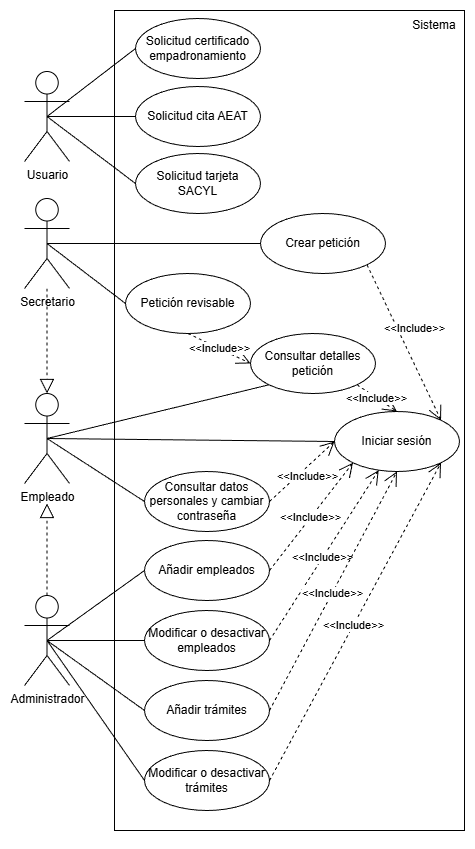
\includegraphics[width=0.6\textwidth]{img/diagramas/diagrama_casos_uso.png}
            \caption{Diagrama de casos de uso.}
        \end{figure}

    \subsection{Actores:}
        \begin{enumerate}
            \item Usuario: persona ajena a la Administración pública que necesita un servicio de la misma.
                Se comunica con el sistema mediante llamadas telefónicas.
            \item Empleados: representa a un trabajador de los organismos públicos. 
                Tienen acceso a la web interna y desempeñan distintas acciones en función de su rol. 
                \begin{itemize}
                    \item Administrador: su función principal es la gestión de empleados y trámites en la plataforma interna.
                    \item Secretario: se encargan de supervisar y completar las peticiones. 
                        También pueden crear peticiones manualmente en caso de que sea necesario, ya sea por subsanar algún error o por cualquier otra razón. 
                \end{itemize}
        \end{enumerate}

    \subsection{Solicitud del certificado de empadronamiento:}
        \begin{longtable}{|p{16cm}|} 
        \hline
        \textbf{Solicitud del certificado de empadronamiento} \\ \hline
        \textbf{Actor principal:} Usuario \\ \hline
        \textbf{Precondición:} El usuario ha iniciado la llamada al sistema \\ \hline
        \textbf{Secuencia normal:} \\
        \begin{minipage}[t]{\linewidth}
            \begin{enumerate}
                \item El usuario solicita obtener el certificado de empadronamiento.
                \item El sistema solicita el DNI.
                \item El usuario proporciona el DNI.
                \item El sistema solicita el nombre.
                \item El usuario proporciona su nombre.
                \item El sistema solicita los dos apellidos.
                \item El usuario proporciona sus dos apellidos.
                \item El sistema solicita el teléfono.
                \item El usuario proporciona su teléfono.
                \item El sistema solicita el motivo de la petición.
                \item El usuario responde el motivo de la petición.
                \item El sistema repite la información obtenida y solicita confirmación. 
                \item El usuario confirma los datos.
                \item El sistema almacena la petición.
                \item El sistema rellena el formulario de solicitud del certificado de empadronamiento con los datos obtenidos.
            \end{enumerate}
            \vspace{1mm}
        \end{minipage} \\ \hline
        \textbf{Flujos alternativos:} \\
        \begin{minipage}[t]{\linewidth}
            \begin{enumerate}
                \item[11.a] Si el usuario no confirma los datos, el sistema repite las preguntas correspondientes y se continúa con el paso siguiente a la pregunta.
            \end{enumerate}
            \vspace{1mm}
        \end{minipage}\\ \hline
        \caption{Descripción general del caso de uso - Solicitud del certificado de empadronamiento.}
        \end{longtable}
        
    \subsection{Solicitud de cita en la Agencia Tributaria:}
        \begin{longtable}{|p{16cm}|} 
        \hline
        \textbf{Solicitud de cita en la Agencia Tributaria} \\ \hline
        \textbf{Actor principal:} Usuario. \\ \hline
        \textbf{Precondición:} El usuario ha iniciado una llamada al sistema. \\ \hline
        \textbf{Secuencia normal:}\\
        \begin{minipage}[t]{\linewidth}
            \begin{enumerate}
                \item El usuario solicita agendar una cita en la Agencia Tributaria.
                \item El sistema solicita el DNI.
                \item El usuario proporciona su DNI.
                \item El sistema solicita el nombre y el primer apellido.
                \item El usuario proporciona su nombre y sus primer apellido.
                \item El sistema solicita el tipo de servicio.
                \item El usuario proporciona el tipo de servicio.
                \item El sistema pregunta si prefiere cita telefónica o presencial.
                \item El usuario responde que presencial.
                \item El sistema solicita la oficina.
                \item El usuario responde la oficina.
                \item El sistema solicita fecha y hora preferible para la cita.
                \item El usuario responde la fecha y hora.
                \item El sistema comprueba que la fecha y hora es válida.
                \item El sistema repite la información obtenida y solicita confirmación. 
                \item El usuario confirma los datos.
                \item El sistema almacena la petición.
                \item El sistema rellena el formulario para agendar la cita.
            \end{enumerate} 
            \vspace{1mm}
        \end{minipage} \\ \hline
        \textbf{Flujos alternativos:} \\
        \begin{minipage}[t]{\linewidth}
            \begin{enumerate}
                \item[9.a.] Si el usuario responde cita telefónica se continúa con el paso 15.
                \item[14.a.] Si la fecha u hora no es válida se vuelve al paso 12.
                \item[16.a] Si el usuario no confirma los datos, el sistema repite las preguntas correspondientes y se continúa con el paso siguiente a la pregunta.
            \end{enumerate}
            \vspace{1mm}
        \end{minipage} \\ \hline
        \caption{Descripción general del caso de uso - Solicitud de cita en la Agencia Tributaria.}
        \end{longtable}
        
    \subsection{Solicitud de la tarjeta sanitaria de SACYL por pérdida o robo:}
        \begin{longtable}{|p{16cm}|} 
        \hline
        \textbf{Solicitud de la tarjeta sanitaria de SACYL por pérdida o robo} \\ \hline
        \textbf{Actor principal:} Usuario. \\ \hline
        \textbf{Precondición:} el usuario ha iniciado una llamada al sistema. \\ \hline
        \textbf{Secuencia normal:} \\
        \begin{minipage}[t]{\linewidth}
            \begin{enumerate}
                \item El usuario solicita la tarjeta sanitaria.
                \item El sistema solicita el motivo (pérdida o robo).
                \item El usuario proporciona el motivo (pérdida o robo).
                \item El sistema solicita el nombre.
                \item El usuario proporciona su nombre.
                \item El sistema solicita el primer apellido.
                \item El usuario proporciona su primer apellido.
                \item El sistema solicita la fecha de nacimiento.
                \item El usuario proporciona su fecha de nacimiento.
                \item El sistema pregunta el centro de salud.
                \item El usuario responde su centro de salud.
                \item El sistema solicita la dirección.
                \item El usuario responde la dirección.
                \item El sistema repite la información obtenida y solicita confirmación. 
                \item El usuario confirma los datos.
                \item El sistema almacena la petición.
                \item El sistema rellena el formulario para solicitar la tarjeta sanitaria.
            \end{enumerate}
            \vspace{1mm}
        \end{minipage} \\ \hline
        \textbf{Flujos alternativos:} \\
        \begin{minipage}[t]{\linewidth}
            \begin{enumerate}
                \item[15.a] Si el usuario no confirma los datos, el sistema repite las preguntas correspondientes y se continúa con el paso siguiente a la pregunta.
            \end{enumerate}
            \vspace{1mm}
        \end{minipage} \\ \hline
        \caption{Descripción general del caso de uso - Solicitud de la tarjeta sanitaria de SACYL por pérdida o robo.}
        \end{longtable}

    \subsection{Iniciar sesión:}
    \label{subsec:2.4.5.}
        \begin{longtable}{|p{16cm}|} 
        \hline
        \textbf{Iniciar sesión} \\ \hline
        \textbf{Actor principal:} Empleado. \\ \hline
        \textbf{Secuencia normal:} \\
        \begin{minipage}[t]{\linewidth}
            \begin{enumerate}
                \item El sistema solicita el usuario o correo electrónico y la contraseña.
                \item El empleado introduce su usuario o correo electrónico y su contraseña.
                \item El sistema comprueba que los datos coinciden con un empleado e inicia sesión.
            \end{enumerate}
            \vspace{1mm}
        \end{minipage} \\ \hline
        \textbf{Flujos alternativos:} \\
        \begin{minipage}[t]{\linewidth}
            \begin{enumerate}
                \item[3.a.] Si los datos no coinciden con un empleado, el sistema informa de datos incorrectos y vuelve al paso 1.
                \item[3.b.] Si los datos coinciden pero el ususario está desactivado, el sistema lo informa y vuelve al paso 1.
            \end{enumerate}
            \vspace{1mm}
        \end{minipage} \\ \hline
        \textbf{Postcondiciones:} el empleado está identificado en el sistema. \\ \hline
        \caption{Descripción general del caso de uso - Iniciar sesión.}
        \end{longtable}

    \subsection{Consultar detalles de una petición:}
    \label{subsec:2.4.6.}
        \begin{longtable}{|p{16cm}|} 
        \hline
        \textbf{Consultar detalles de una petición} \\ \hline
        \textbf{Actor principal:} Empleado. \\ \hline
        \textbf{Precondición:} caso de uso \hyperref[subsec:2.4.5.]{2.4.5. Inicia sesión}. \\ \hline
        \textbf{Secuencia normal:} \\
        \begin{minipage}[t]{\linewidth}
            \begin{enumerate}
                \item El empleado va a la página con la lista de peticiones.
                \item El empleado clica en el ID de la petición.
                \item El sistema muestra la información de la petición.
            \end{enumerate}
            \vspace{1mm}
        \end{minipage} \\ \hline
        \caption{Descripción general del caso de uso - Consultar detalles de una petición.}
        \end{longtable}

    \subsection{Petición revisable:}
        \begin{longtable}{|p{16cm}|} 
        \hline
        \textbf{Petición revisable} \\ \hline
        \textbf{Actor principal:} Secretario. \\ \hline
        \textbf{Precondición:} caso de uso \hyperref[subsec:2.4.6.]{2.4.6. Consultar detalles de una petición}. \\ \hline
        \textbf{Secuencia normal:} \\
        \begin{minipage}[t]{\linewidth}
            \begin{enumerate}
                \item El secretario se asigna la petición.
                \item El secretario modifica la información necesaria.
                \item El secretario completa la petición.
                \item El sistema inicia el trámite correspondiente a la petición.
                \item El sistema actualiza el estado de la petición a completada. 
            \end{enumerate}
            \vspace{1mm}
        \end{minipage} \\ \hline
        \textbf{Flujos alternativos:} \\
        \begin{minipage}[t]{\linewidth}
            \begin{enumerate}
                \item[3.a.] Si el secretario anula la petición, cambia y actualiza el estado a cancelada y finaliza el caso de uso. 
            \end{enumerate}
            \vspace{1mm}
        \end{minipage} \\ \hline
        \caption{Descripción general del caso de uso - Petición revisable.}
        \end{longtable}

    \subsection{Consultar datos personales y cambiar contraseña:}
        \begin{longtable}{|p{16cm}|} 
        \hline
        \textbf{Consultar datos personales y cambiar contraseña} \\ \hline
        \textbf{Actor principal:} Empleado. \\ \hline
        \textbf{Precondición:} caso de uso \hyperref[subsec:2.4.5.]{2.4.5. Inicia sesión}. \\ \hline
        \textbf{Secuencia normal:} \\
        \begin{minipage}[t]{\linewidth}
            \begin{enumerate}
                \item El empleado clica en su perfil.
                \item El sistema muestra su información personal.
                \item El empleado clica en cambiar contraseña.
                \item El sistema solicita la contraseña actual y la contraseña nueva.
                \item El empleado introduce la información.
                \item El sistema comprueba que la contraseña actual es verídica.
                \item El sistema actualiza la contraseña del empleado.
            \end{enumerate}
            \vspace{1mm}
        \end{minipage} \\ \hline
        \textbf{Flujos alternativos:} \\
        \begin{minipage}[t]{\linewidth}
            \begin{enumerate}
                \item[6.a.] Si la contraseña actual es incorrecta, el sistema lo informa y vuelve al paso 4.
            \end{enumerate}
            \vspace{1mm}
        \end{minipage} \\ \hline
        \caption{Descripción general del caso de uso - Consultar datos personales y cambiar contraseña.}
        \end{longtable}

    \subsection{Crear petición:}
        \begin{longtable}{|p{16cm}|} 
        \hline
        \textbf{Crear petición} \\ \hline
        \textbf{Actor principal:} Secretario. \\ \hline
        \textbf{Precondición:} caso de uso \hyperref[subsec:2.4.5.]{2.4.5. Inicia sesión}. \\ \hline
        \textbf{Secuencia normal:} \\
        \begin{minipage}[t]{\linewidth}
            \begin{enumerate}
                \item El secretario va a la página con la lista de peticiones.
                \item El secretario clica en crear petición.
                \item El sistema solicita el teléfono y el trámite.
                \item El secretario introduce el teléfono y el trámite.
                \item El sistema solicita la información correspondiente al trámite.
                \item El secretario introduce la información.
                \item El sistema crea la petición e inicia el trámite.
            \end{enumerate}
            \vspace{1mm}
        \end{minipage} \\ \hline
        \caption{Descripción general del caso de uso - Crear petición.}
        \end{longtable}

    \subsection{Añadir empleados:}
        \begin{longtable}{|p{16cm}|} 
        \hline
        \textbf{Añadir empleados} \\ \hline
        \textbf{Actor principal:} Administrador. \\ \hline
        \textbf{Precondición:} caso de uso \hyperref[subsec:2.4.5.]{2.4.5. Inicia sesión}. \\ \hline
        \textbf{Secuencia normal:} \\
        \begin{minipage}[t]{\linewidth}
            \begin{enumerate}
                \item El administrador va a la página con la lista de empleados.
                \item El administrador selecciona añadir empleado.
                \item El sistema solicita los datos del nuevo empleado.
                \item El administrador rellena los datos.
                \item El sistema comprueba que el email no está registrado ya en el sistema.
                \item El sistema crea un usuario y una contraseña temporal.
                \item El sistema envía al nuevo usuario su contraseña temporal.
                \item El sistema almacena el nuevo empleado.
            \end{enumerate}
            \vspace{1mm}
        \end{minipage} \\ \hline
        \textbf{Flujos alternativos:} \\
        \begin{minipage}[t]{\linewidth}
            \begin{enumerate}
                \item[5.a.] Si el email ya está registrado, el sistema lo informa y continúa con el paso 3.
            \end{enumerate}
            \vspace{1mm}
        \end{minipage} \\ \hline
        \caption{Descripción general del caso de uso - Añadir empleados.}
        \end{longtable}

    \subsection{Modificar o desactivar empleados}
        \begin{longtable}{|p{16cm}|} 
        \hline
        \textbf{Modificar o desactivar empleados} \\ \hline
        \textbf{Actor principal:} Administrador. \\ \hline
        \textbf{Precondición:} caso de uso \hyperref[subsec:2.4.5.]{2.4.5. Inicia sesión}. \\ \hline
        \textbf{Secuencia normal:} \\
        \begin{minipage}[t]{\linewidth}
            \begin{enumerate}
                \item El administrador va a la página con la lista de empleados.
                \item El administrador clica en el botón de la columna activo del empleado correspondiente.
                \item El sistema muestra los campos con la información del empleado.
                \item El administrador modifica la información correspondiente y clica en editar.
                \item El sistema actualiza la información del empleado.
            \end{enumerate}
            \vspace{1mm}
        \end{minipage} \\ \hline
        \textbf{Flujos alternativos:} \\
        \begin{minipage}[t]{\linewidth}
            \begin{enumerate}
                \item[3.a.] El administrador clica en resetear contraseña, el sistema crea una contraseña temporal y se la envía al email del empleado.
                \item[4.a.] El administrador modifica el email, el sistema comprueba que el email ya está registrado en el sistema, lo informa y vuelve al paso 3.
                \item[4.b.] El administrador modifica el email, el sistema comprueba que el email no está registrado en el sistema y continúa con el paso 5.
                \item[4.c.] El administrador activa o desactiva el empleado, el sistema se lo avisa al email del empleado y continúa en el paso 5.
            \end{enumerate}
            \vspace{1mm}
        \end{minipage} \\ \hline
        \caption{Descripción general del caso de uso - Modificar o desactivar empleados.}
        \end{longtable}

    \subsection{Añadir trámites:}
        \begin{longtable}{|p{16cm}|} 
        \hline
        \textbf{Añadir trámites} \\ \hline
        \textbf{Actor principal:} Administrador. \\ \hline
        \textbf{Precondición:} caso de uso \hyperref[subsec:2.4.5.]{2.4.5. Inicia sesión}. \\ \hline
        \textbf{Secuencia normal:} \\
        \begin{minipage}[t]{\linewidth}
            \begin{enumerate}
                \item El administrador va a la página con la lista de trámites.
                \item El administrador clica en añadir trámite.
                \item El sistema solicita el nombre y estado del trámite.
                \item El administrador introduce el nombre y estado del trámite.
                \item El sistema comprueba que no hay otro trámite con el mismo nombre.
                \item El sistema actualiza los datos del trámite.
            \end{enumerate}
            \vspace{1mm}
        \end{minipage} \\ \hline
        \textbf{Flujos alternativos:} \\
        \begin{minipage}[t]{\linewidth}
            \begin{enumerate}
                \item[5.a.] El sistema comprueba que hay otro trámite con el mismo nombre, lo informa y vuelve al paso 3.
            \end{enumerate}
            \vspace{1mm}
        \end{minipage} \\ \hline
        \caption{Descripción general del caso de uso - Añadir trámites.}
        \end{longtable}

    \subsection{Modificar o desactivar trámites:}
        \begin{longtable}{|p{16cm}|} 
        \hline
        \textbf{Modificar o desactivar trámites} \\ \hline
        \textbf{Actor principal:} Administrador. \\ \hline
        \textbf{Precondición:} caso de uso \hyperref[subsec:2.4.5.]{2.4.5. Inicia sesión}. \\ \hline
        \textbf{Secuencia normal:} \\
        \begin{minipage}[t]{\linewidth}
            \begin{enumerate}
                \item El administrador va a la página con la lista de trámites.
                \item El administrador clica en el botón de la columna activo del trámite correspondiente.
                \item El sistema muestra los campos con la información del trámite.
                \item El administrador modifica la información correspondiente y clica en editar.
                \item El sistema actualiza la información del trámite.
            \end{enumerate}
            \vspace{1mm}
        \end{minipage} \\ \hline
        \textbf{Flujos alternativos:} \\
        \begin{minipage}[t]{\linewidth}
            \begin{enumerate}
                \item[4.a.] El administrador modifica el título del trámite, el sistema comprueba que el título ya está registrado en el sistema, lo informa y vuelve al paso 3.
                \item[4.b.] El administrador modifica el título del trámite, el sistema comprueba que el título no está registrado en el sistema y continúa con el paso 5.
                \item[4.c.] Si el administrador desactiva un trámite activo, el sistema cancela todas las peticiones no completadas de ese trámite y va al paso 5.
            \end{enumerate}
            \vspace{1mm}
        \end{minipage} \\ \hline
        \caption{Descripción general del caso de uso - Modificar o desactivar trámites.}
        \end{longtable}
    
\section{Modelo de dominio:}
    \begin{figure}[H]
        \centering
        
\includegraphics[width=0.8\textwidth]{img/diagramas/modelo_dominio.png}
        \caption{Modelo de dominio.}
    \end{figure}

\chapter{Planificación}
\section{Metodología}
    Para el desarrollo del proyecto se ha seguido un modelo de desarrollo estructural en cascada. 
    Este enfoque divide el proceso de desarrollo en fases claramente diferenciadas que se suceden de forma secuencial, comenzando cada fase una vez finalizada la anterior. 

    Las fases típicas de este modelo incluyen el análisis, el diseño, la implementación, las pruebas y el mantenimiento. 
    No obstante, al tratarse de un proyecto académico, la fase de mantenimiento no es necesaria y se sustituye por la documentación final de la memoria.

    Se emplea esta metodología debido a que el objetivo final del proyecto está claramente definido desde el inicio, con unos requisitos bien establecidos y sin necesidad de iteraciones incrementales. 
    Por ello, la planificación del proyecto se ha realizado tomando como base el análisis inicial, permitiendo organizar de forma coherente y estructural el desarrollo del trabajo.

\section{Planificación temporal}
    La organización temporal del proyecto se ha realizado siguiendo la dedicación exigida por la guía docente de la asignatura \cite{guiadocente-tfg}.
    El proyecto se ha planificado para ser elaborado en un total de 300 horas, distribuidas en 15 semanas, dedicando aproximadamente 20 horas semanales al desarrollo del mismo. 
    Se ha repartido el trabajo en 6 fases, estructuradas temporalmente según la Tabla \ref{tab:3.1}.

    \begin{table}[H]
        \centering
        \begin{tabular}{|c c c >{\centering\arraybackslash}p{8cm}|}
        \hline
        \textbf{Fase} & \textbf{Semanas} & \textbf{Horas} & \textbf{Entregables} \\ \hline
        Análisis & 1 & 10 & Estudio del alcance de la aplicación, definición de requisitos y casos de uso\\
        Planificación & 1 & 10 & Planificación temporal y seguimiento del proyecto\\
        Diseño & 2 & 20 & Decisiones técnicas, diagramas UML, diseño de la base de datos y mockups\\
        Implementación & 3-8 & 120 & Sistema funcional\\
        Pruebas & 8-9 & 40 & Validación del sistema\\
        Documentación & 10-15 & 100 & Memoria final y presentación\\
        \hline
        \end{tabular}
        \caption{Planificación temporal inicial del proyecto.}
        \label{tab:3.1}
    \end{table}

\section{Estimación de costes}
    La estimación de costes se ha realizado considerando el tiempo de dedicación al proyecto y el coste asociado a la hora de trabajo.
    El coste de un desarrollador junior se sitúa aproximadamente en 15€/h, lo que supone un coste total estimado de 4500€ para las 300 horas de trabajo planificadas. 

    Durante la fase de desarrollo no se prevén costes adicionales, ya que se utilizarán herramientas gratuitas y servicios que ofrecen planes con créditos gratuitos suficientes para cubrir las necesidades del proyecto.

\section{Análisis de riesgos}
    En esta sección se muestran los principales riesgos identificados durante la planificación del proyecto, junto con su probabilidad de ocurrencia, su impacto y las posibles medidas para mitigarlos, Talba \ref{tab:3.3}. 

    \begin{table}[H]
        \centering
        \begin{tabular}{| p{4.5cm} | c | c | p{7cm} |}
            \hline
            \textbf{Riesgo} & \textbf{Probabilidad} & \textbf{Impacto} & \textbf{Salvaguarda} \\ \hline
            Créditos insuficientes en servicios en la nube & Media & Alto & Monitorización del gasto de créditos y evitar el uso innecesario de recursos. \\ \hline
            Incremento inesperado del coste de las tecnologías utilizadas & Baja & Medio & Evaluación continua de los costes asociados y búsqueda de alternativas gratuitas o de bajo coste. \\ \hline
            Indisponibilidad temporal de los servicios externos & Baja & Alto & Uso de servicios consolidados con buen soporte. \\ \hline
            Aparición de imprevistos que afecten al tiempo de desarrollo & Alta & Medio & Planificación de tiempo adicional para imprevistos y margen con la fecha límite de entrega. \\ \hline
            Complejidad técnica en la integración de los distintos componentes del sistema & Media & Medio & Formación y estudio previo de las tecnologías utilizadas. \\ \hline
        \end{tabular}
        \caption{Análisis de riesgos del proyecto.}
        \label{tab:3.2}
    \end{table}

\section{Seguimiento del proyecto}
    A lo largo del desarrollo del proyecto, se ha llevado un seguimiento detallado para controlar el gasto temporal real frente al planificado. 
    En la Tabla \ref{tab:3.3} se muestra la comparativa entre la planificación temporal inicial y el progreso real del proyecto, permitiendo identificar desajustes y calcular el coste real del proyecto.
    \begin{table}[H]
        \centering
        \begin{tabular}{|c c c | c|}
            \hline
            \textbf{Fase} & \textbf{Horas Programadas} & \textbf{Horas Reales} \\ \hline
            Análisis & 10 & 15 \\
            Planificación & 10 & 8 \\
            Diseño & 20 & 25 \\
            Implementación & 120 & 180 \\
            Pruebas & 40 & 35 \\
            Documentación & 100 & 90\\
            \hline
        \end{tabular}
        \caption{Seguimiento del proyecto.}
        \label{tab:3.3}
    \end{table}
    El gasto temporal real del proyecto asciende a 353 horas por imprevistos en la fase de implementación. 
    
    Inicialmente, estaba previsto el uso de la red telefónica para la comunicación entre los usuarios y el sistema, lo que no aumentaba el gasto temporal ya que venía integrado con los servicios de la IA.
    Sin embargo, debido al elevado coste de esta solución en desarrollo, se optó por una solución basada en llamadas VoIP, que resulta completamente gratuita, pero implica un desarrollo adicional para integrar esta funcionalidad en el sistema.

    En cuanto al coste real del proyecto, el gasto ascendería a 5295€, superando el presupuesto inicial en 795€. 
    El gasto de la red telefónica hubiera supuesto un coste adicional de 1,50€ de establecimiento de llamada más 1€ adicional por cada minuto. 
    Además, el coste de alquiler de una línea telefónica virtual hubiera implicado un gasto mensual de entre 5-10€/mes. 
    Estos gastos hubieran complicado el desarrollo del proyecto, limitando el número de llamadas que se podrían realizar durante la fase de implementación y pruebas, lo que hubiera afectado negativamente a la calidad del sistema.

\chapter{Diseño}
\section{Decisiones técnicas}
    En esta sección se plantean las herramientas y tecnologías que se van a utilizar para llevar a cabo el desarrollo del proyecto, justificando cada una de ellas.
    
    \subsection{Frontend} 
        Para programar el frontend de la aplicación web para empleados se utilizará HTML, CSS y JavaScript. 
        Se usará también Jinja2, un motor de plantillas integrado con Flask que permite generar HTML de manera dinámica.
     
    \subsection{Backend}
        Para programar la lógica del backend de la aplicación se utilizará Python. 
        Servirá de conexión entre Dialogflow, la base de datos y la aplicación web. 
            
        Se utilizará este lenguaje por su flexibilidad y facilidad para integrar todos los servicios. Algunas de las librerías que se emplearán son:
        \begin{itemize}
            \item Flask: framework web para crear aplicaciones web. Se utilizará para desarrollar el backend de la aplicación.
            \item SQLAlchemy: sirve para interactuar con la base de datos SQLite de manera sencilla y eficiente.
            \item Discord.py: librería para interactuar con Discord y programar el bot que atenderá las llamadas VoIP.
            \item Google-Cloud-Dialogflow y Google-Cloud-Speech: para interactuar con los servicios de IA de Google Cloud.
            \item Selenium: para automatizar la simulación de los trámites en las webs oficiales.
        \end{itemize}

    \subsection{Base de datos}
        SQLite es el lenguaje elegido para programar la base de datos ya que está integrado con Python y es suficiente para almacenar la información de nuestro sistema simulado. 

    \subsection{Servicios}
        Algunas de las herramientas y servicios externos que se van a utilizar son:
        \begin{itemize}
            \item Google Cloud: se va a utilizar esta plataforma en la nube para alojar los diferentes servicios de inteligencia artificial del proyecto.
                Se prefiere esta opción frente a otras alternativas ya que integra un servicio propio de agentes conversacionales, ofreciendo un plan gratuito suficiente para el desarrollo.
                \begin{itemize}
                    \item Dialogflow ES: es la herramienta de Google Cloud para crear agentes conversacionales capaces de interpretar el lenguaje natural y las intenciones del usuario mediante algoritmos de machine learning. 
                        Se utilizará para definir las intenciones y los flujos de conversación que podrán tener los usuarios con el agente, recopilar la información requerida para los trámites y devolver el audio a reproducir en la llamada.
                        Esta opción es la más adecuada para proyectos pequeños con pocos trámites.
                    \item Goolge Speech-to-Text: servicio de reconocimiento de voz que convierte el audio de las llamadas VoIP en texto para que pueda ser procesado por Dialogflow. 
                        También se implementará un servicio speech-to-text local con Vosk para poder hacer consultas en desarrollo sin gastos de créditos de Google Cloud.
                \end{itemize}
            \item Discord: es una plataforma de comunicación que permite llamadas VoIP, se usará por la facilidad para crear aplicaciones y bots fácilmente programable en python.
                El usuario iniciará una llamada uniéndose a un canal de Discord y el bot comenzará una conversación conectándose con las IA de Google Cloud.
            \item Gitlab: se usará un control de versiones para mantener actualizados todos los cambios en el código y la documentación del proyecto, y poder recuperar cualquier versión ante un imprevisto. 
            \item Ngrok: crea un túnel desde el despliegue local para tener un endpoint público en desarrollo, necesario para comunicar el backend con Dialogflow. 
                Es una herramienta segura que evita los costes de mantener un servidor propio para la implementación del proyecto, manteniéndonos dentro del alcance definido.
        \end{itemize}
    
    \subsection{Documentación}
        Para la documentación del proyecto se utilizarán las siguientes herramientas:
        \begin{itemize}
            \item Figma: herramienta de diseño para crear los mockups de la interfaz de usuario.
            \item Draw.io: es una herramienta de diseño para crear los diagramas fácilmente para la memoria.
            \item Latex: como sistema de composición de textos para escribir la memoria.
        \end{itemize}

\section{Diseño de la interfaz de usuario}
    En esta sección se muestra el diseño adoptado en la interfaz de la aplicación web destinada a trabajadores de las Administraciones públicas.
    El concepto general de la interfaz se ha centrado en mostrar únicamente la información y funcionalidades necesarias en pantalla, manteniendo un estilo simple y claro que favorece la eficiencia y eficacia en el uso de la aplicación.

    A continuación se presentan los mockups de las páginas principales del sistema.
    En cada prototipo se describen los elementos que lo componen, explicando las funcionalidades que disponen los empleados.

    \begin{figure}[H]
        \centering
        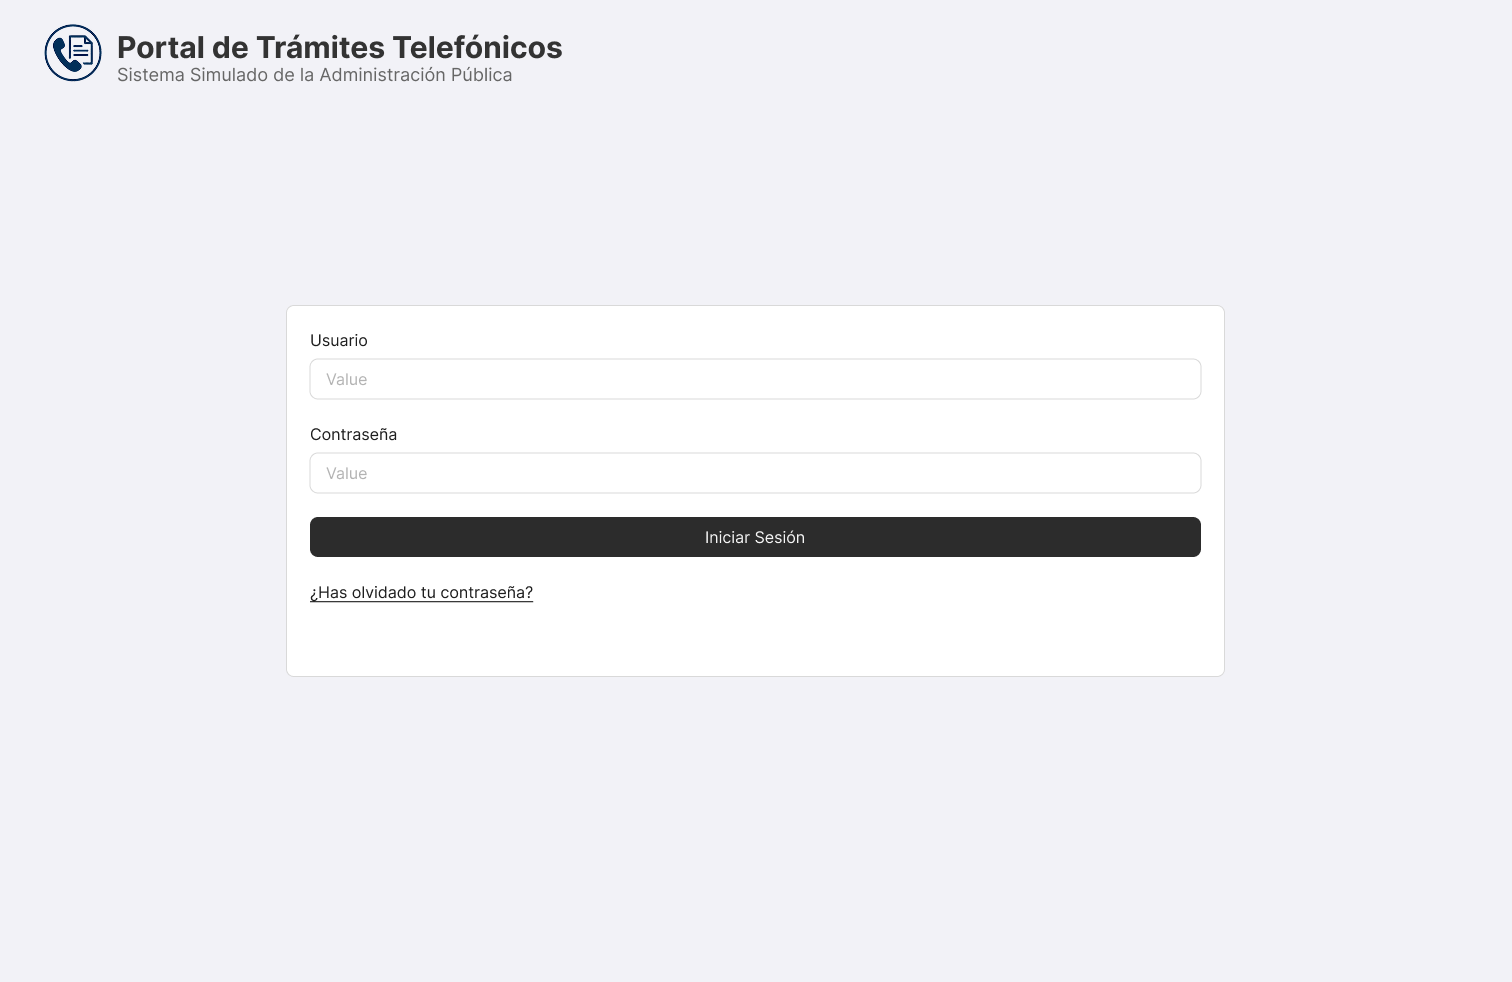
\includegraphics[width=0.8\textwidth]{img/mockups/Login.png}
        \caption{Prototipo visual de la página de login.}
        \label{fig:4.1}
    \end{figure}
    La figura \ref{fig:4.1} muestra la pantalla de inicio de sesión del sistema. 
    Se trata de la página inicial de la aplicación y la única accesible públicamente para usuarios ajenos al sistema.
    Por ello, presenta únicamente un formulario de acceso en la parte central, que permite a los empleados identificarse fácilmente mediante sus credenciales.
        
    Para acceder a cualquier otra página del sistema es necesario autenticarse para garantizar la confidencialidad de la información.

    \begin{figure}[H]
        \centering
        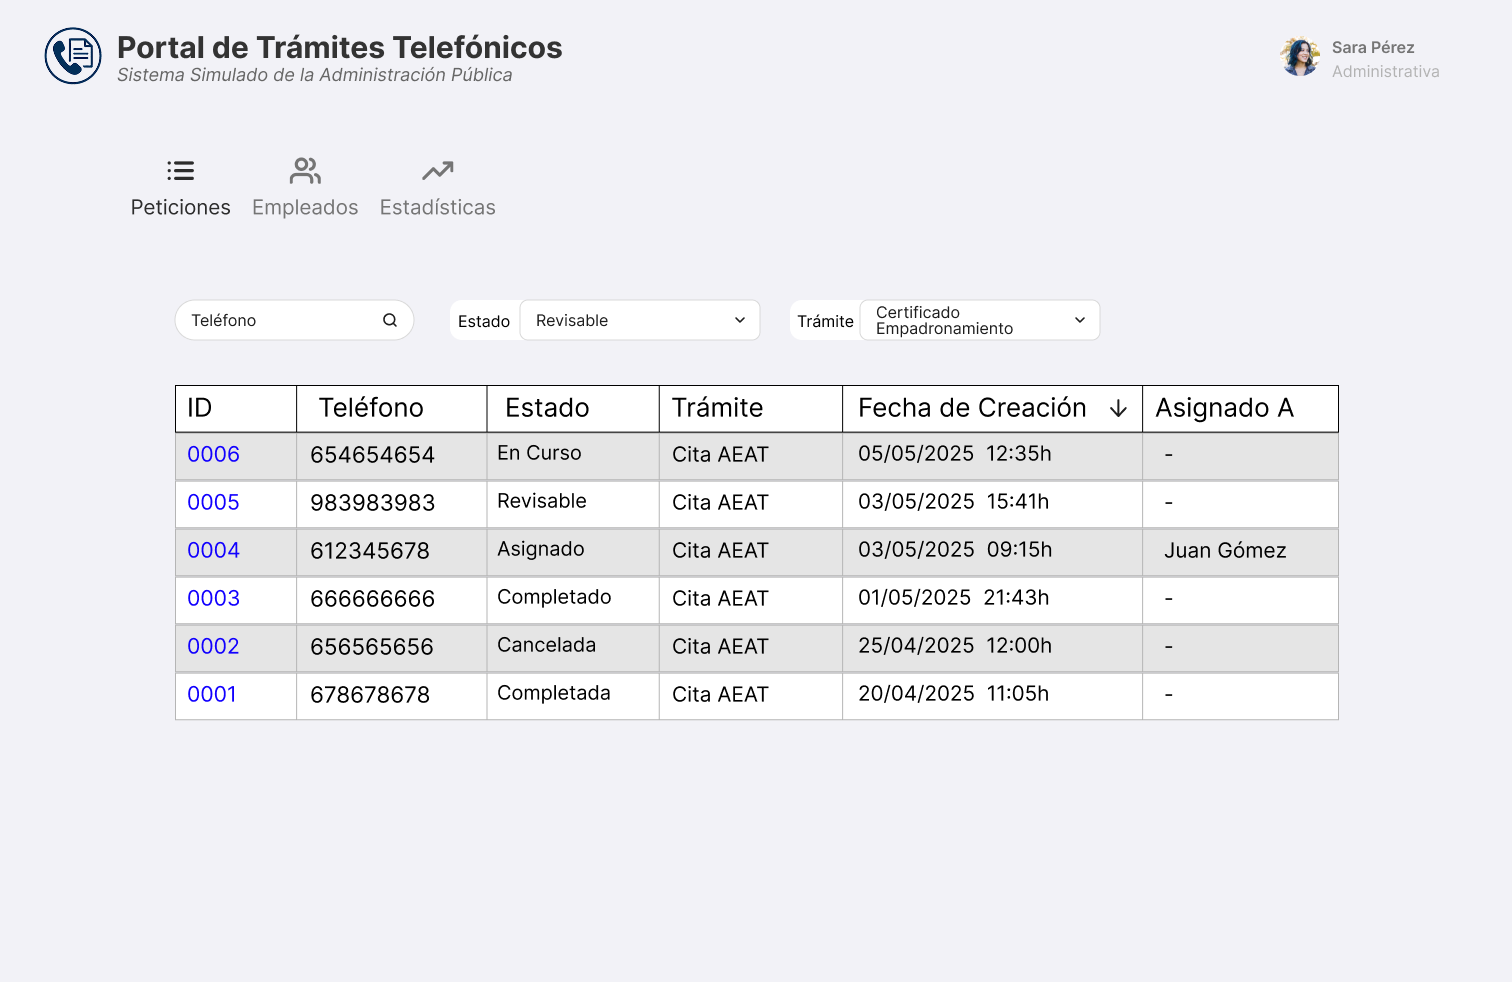
\includegraphics[width=0.8\textwidth]{img/mockups/Peticiones.png}
        \caption{Prototipo visual de la página de peticiones.}
        \label{fig:4.2}
    \end{figure}
    La figura \ref{fig:4.2} muestra un listado con todas las peticiones del sistema. 
    Se trata de la página principal de la aplicación, ya que es visible por todos los empleados.
        
    El componente principal es una tabla con la información básica de cada petición, incluyendo en la parte superior de la tabla una serie de filtros para localizar rápidamente la gestión deseada.
    En cada fila de la tabla se incluye un link, situado en la columna con del ID, para navegar a una página con detalles específicos de cada petición.
    Además, en la parte superior izquierda, debajo del logotipo, se incluye un menú para navegar entre las distintas páginas. 
        
    Por último, todas las páginas incluyen el perfil del empleado identificado en la parte superior derecha. 
    Clicando sobre el perfil se puede navegar hasta la página con detalles del empleado.

    \begin{figure}[H]
        \centering
        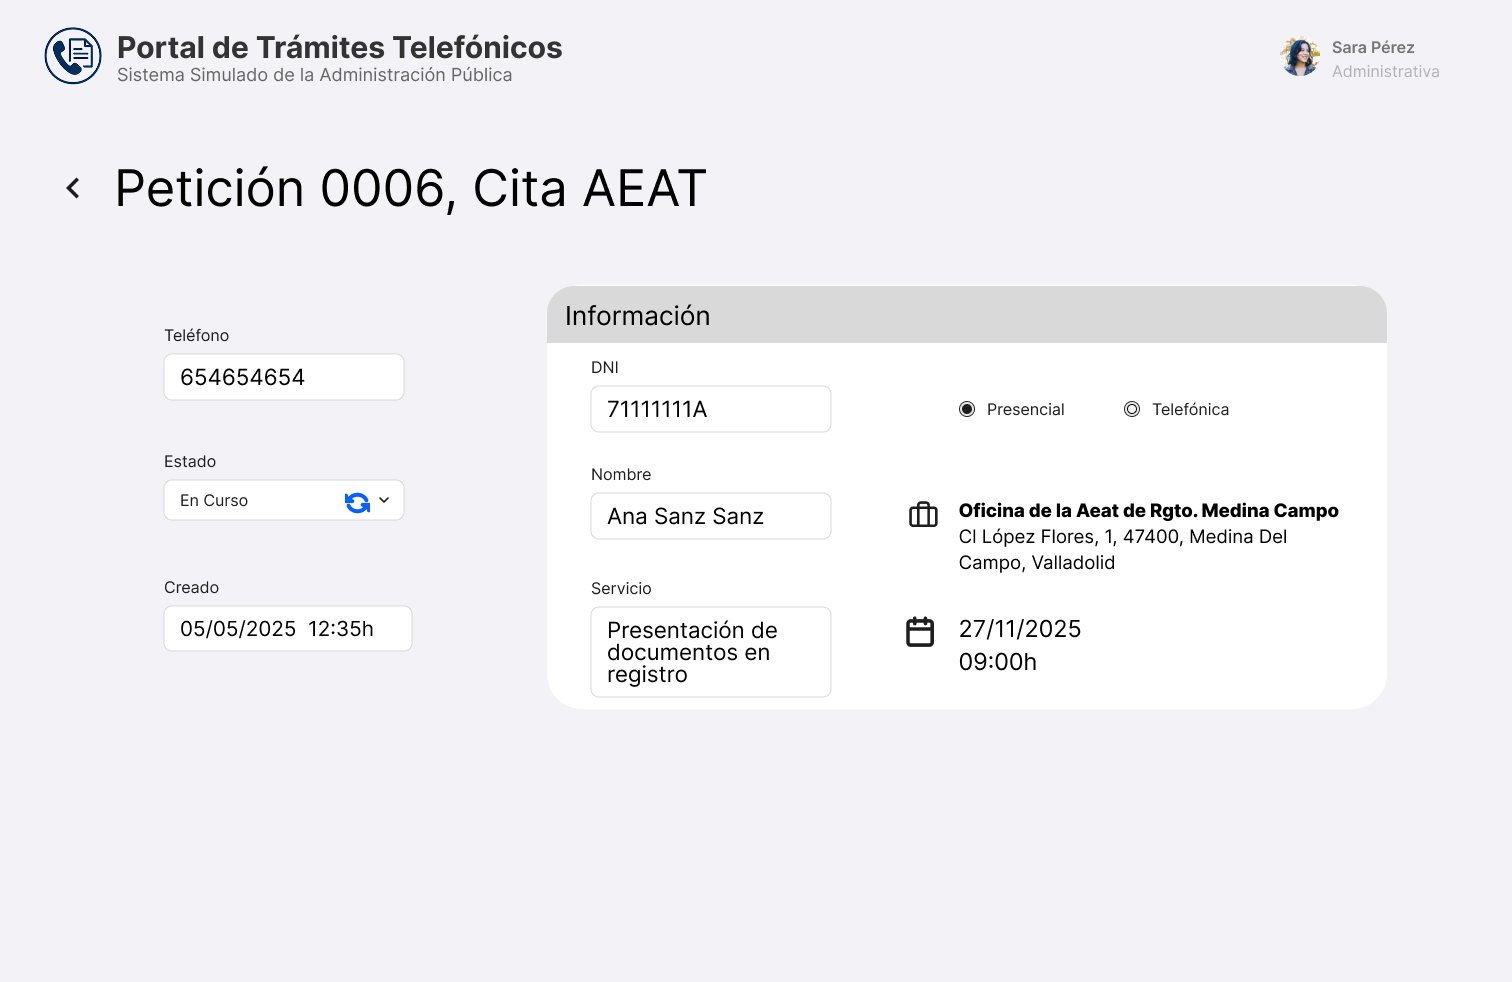
\includegraphics[width=0.8\textwidth]{img/mockups/Peticion.png}
        \caption{Prototipo visual de la página con detalles de una petición.}
        \label{fig:4.3}
    \end{figure}
    \begin{figure}[H]
        \centering
        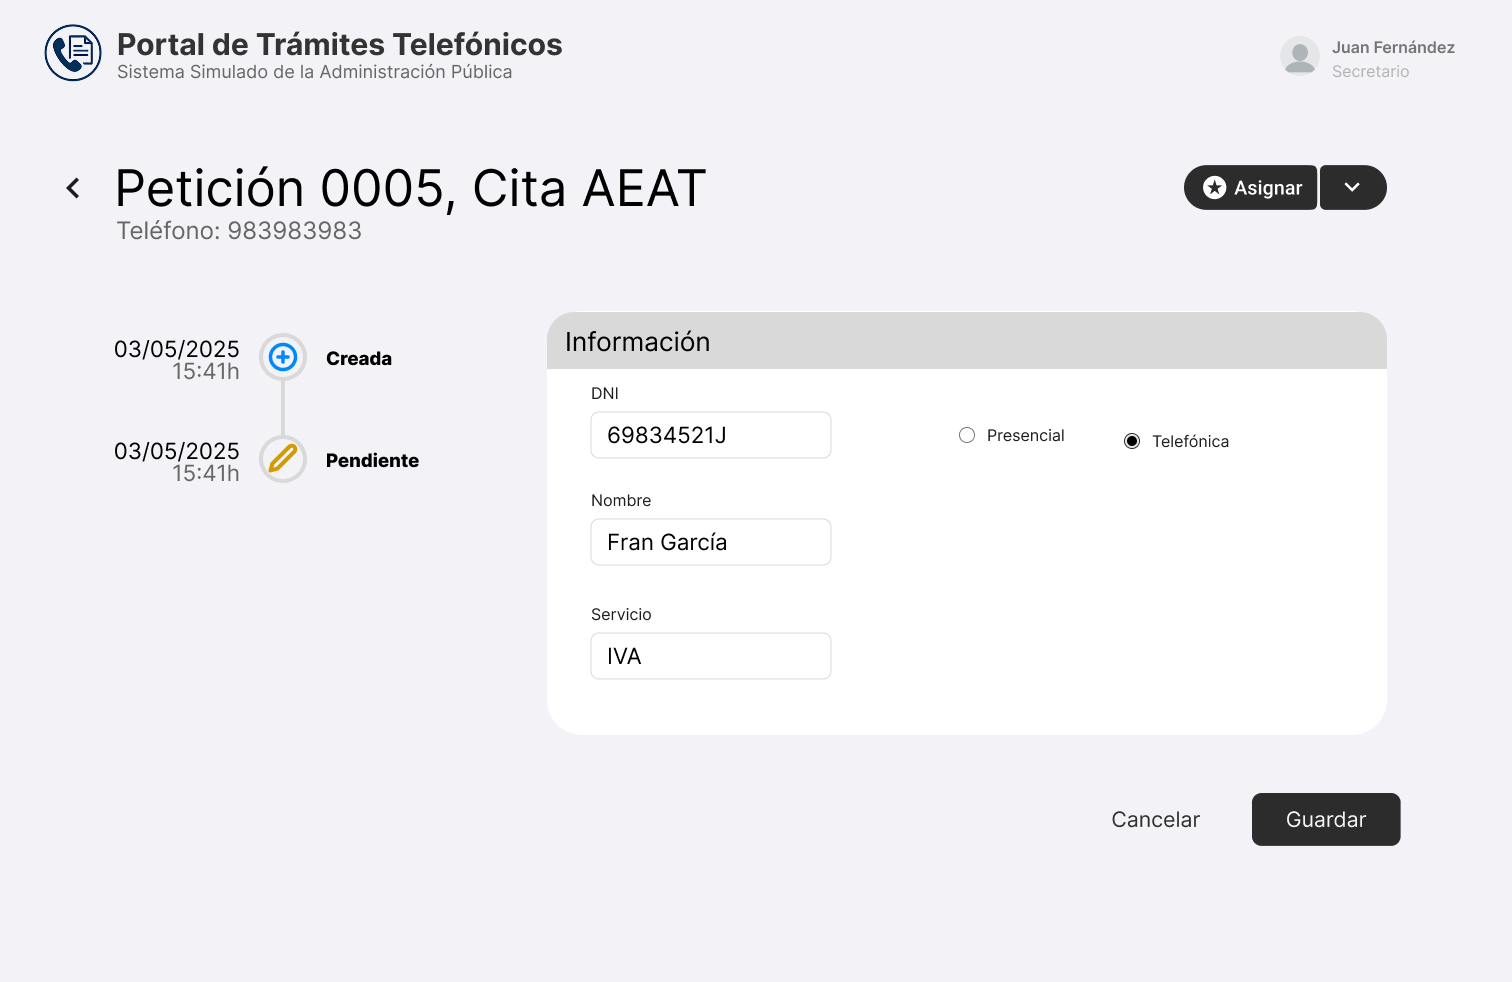
\includegraphics[width=0.8\textwidth]{img/mockups/Revisable.png}
        \caption{Prototipo visual de la página de una petición revisable.}
        \label{fig:4.4}
    \end{figure}
    Al clicar en el ID de una petición en la tabla de la imagen \ref{fig:4.2}, se muestra la página con detalles de la figura \ref{fig:4.3}.
    En esta pantalla se podrá consultar los datos concretos de una petición para cada trámite. 
        
    En caso de ser una petición revisable, figura \ref{fig:4.4}, los empleados que tengan permiso, verán a la derecha del título de la petición un botón para asignársela.
    Una vez asignada, los campos con la información se volverán modificables y los trabajadores podrán editar la petición o cancelarla.
        
    \begin{figure}[H]
        \centering
        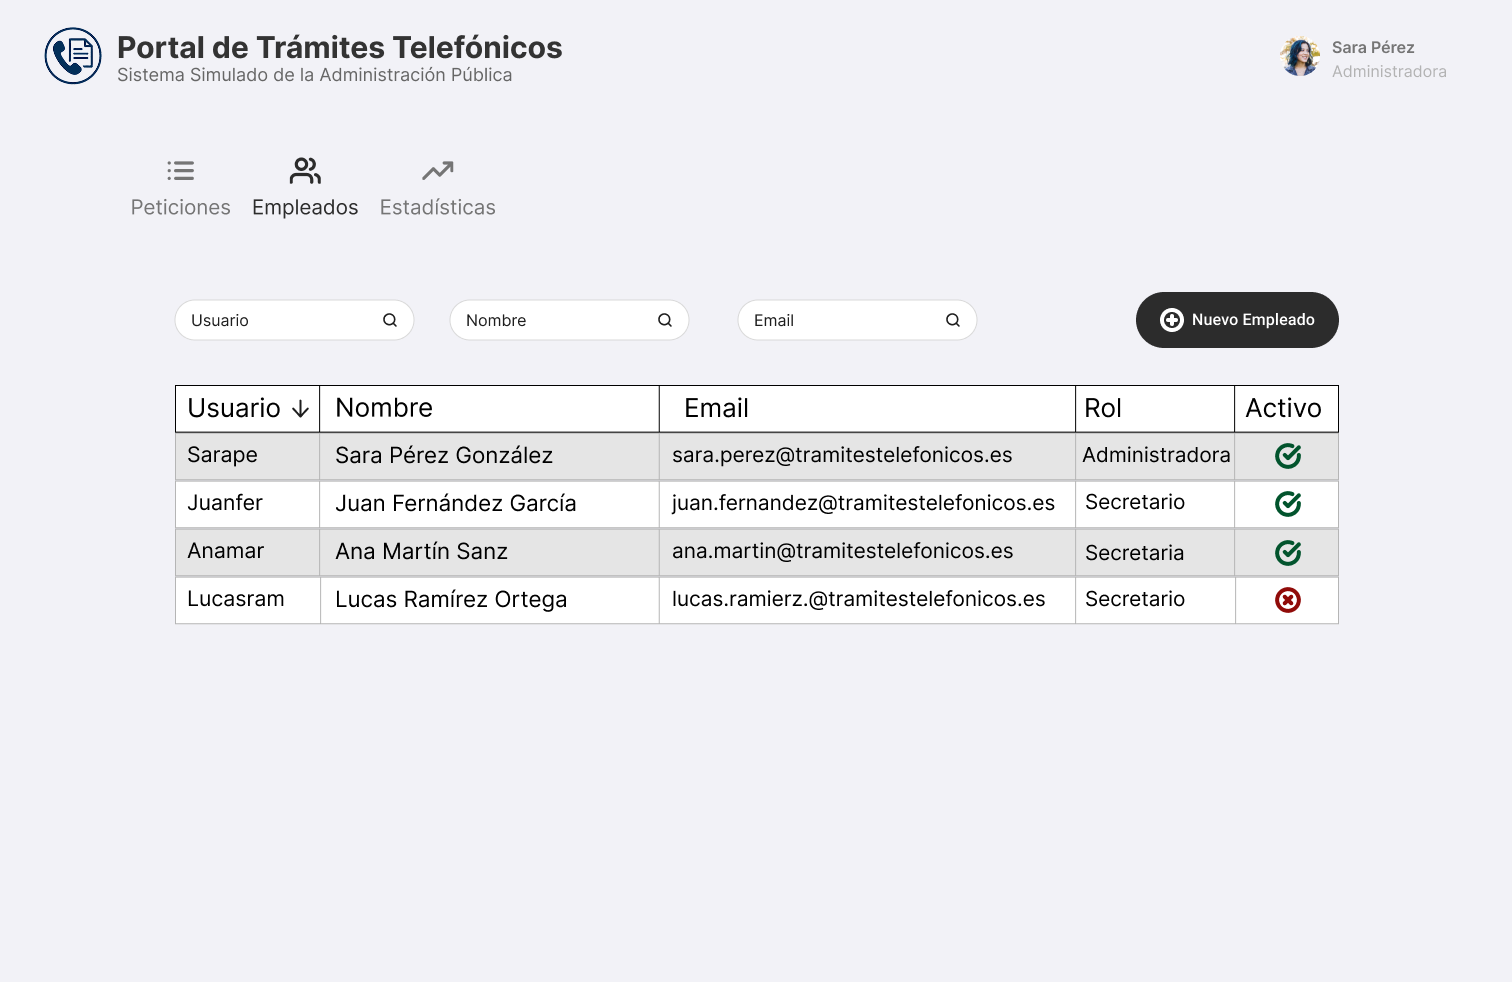
\includegraphics[width=0.8\textwidth]{img/mockups/Empleados.png}
        \caption{Prototipo visual de la página de empleados.}
        \label{fig:4.5}
    \end{figure}
    Desde el menú superior, los administradores pueden navegar hasta la figura \ref{fig:4.5}, que muestra un listado con todos los empleados del sistema. 
    El componente principal es una tabla similar a la de las peticiones, que incluye la información de cada empleado y los filtros necesarios para localizarlos rápidamente.
        
    A diferencia de la otra tabla, se añade una columna que indica si la cuenta de cada empleado está activa. 
    Esta columna cumple una doble función, ya que, clicando sobre el valor correspondiente a un empleado, se navegará hasta una página donde se muestra su información, permitiendo modificarla.
        
    La posibilidad de desactivar cuentas impide el acceso al sistema de un empleado sin necesidad de eliminar su cuenta, perservando así la trazabilidad de la información.
        
    Por último, se incluye a la derecha de los filtros el botón para poder agregar nuevos empleados al sistema.
        
    La página que muestra la información de los trámites será exactamente igual a esta, manteniendo los mismos componenetes, disposición y funcionalidad.

    \begin{figure}[H]
        \centering
        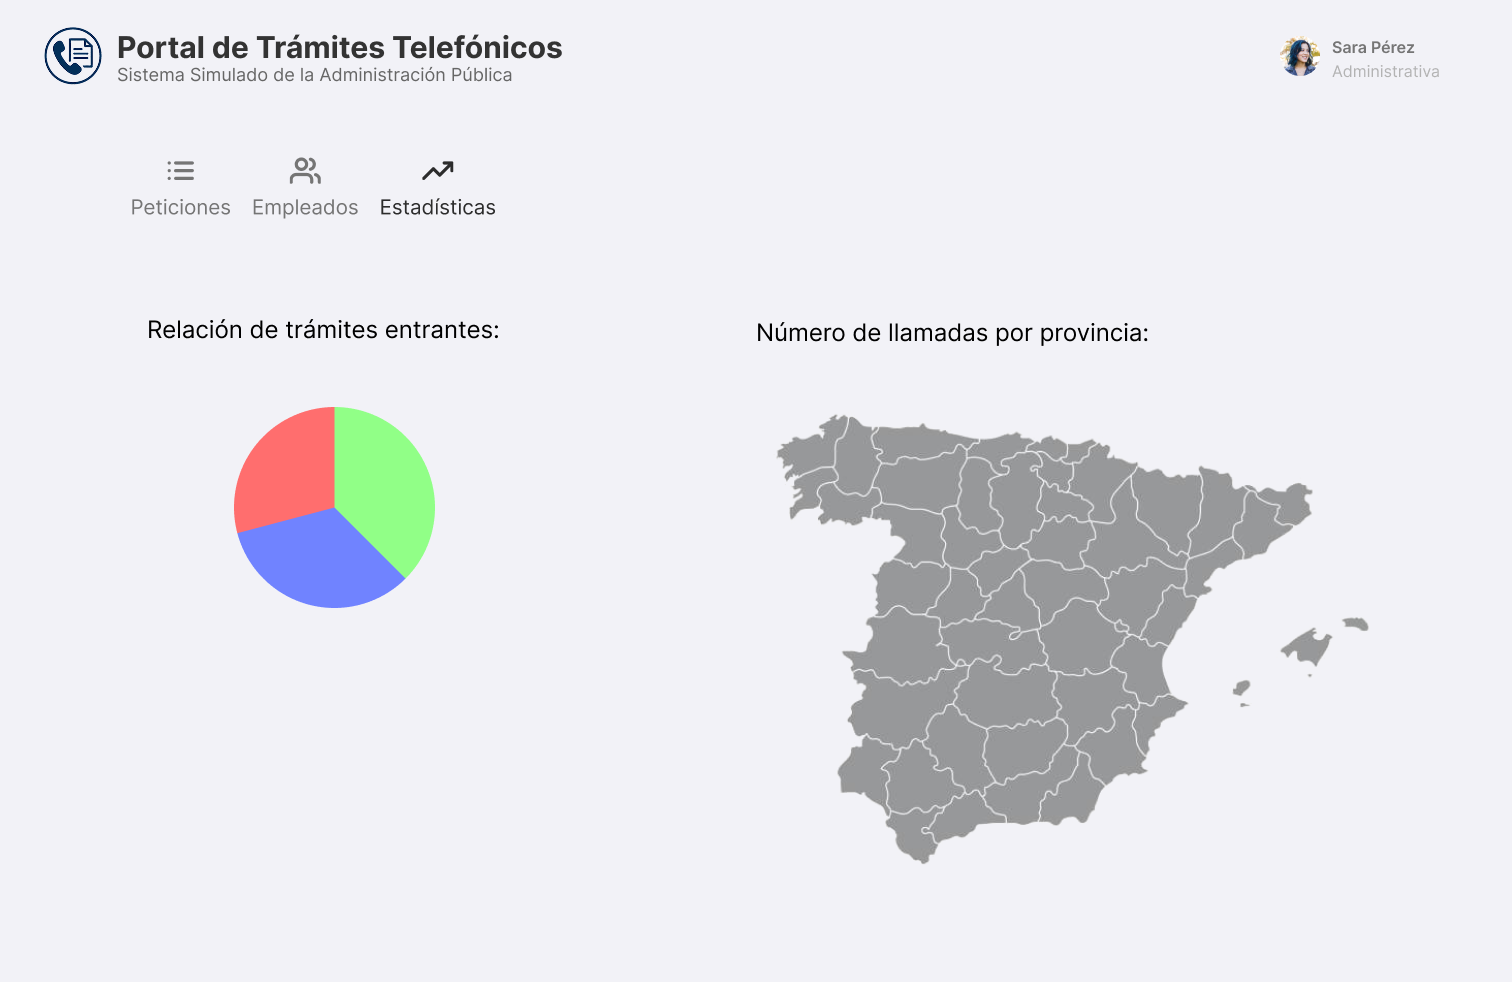
\includegraphics[width=0.8\textwidth]{img/mockups/Estadisticas.png}
        \caption{Prototipo visual de la página de estadísticas.}
        \label{fig:4.6}
    \end{figure}
    Desde el menú de navegación, también se puede acceder a una sección de estadísticas.
    Esta página está diseñada para mostrar información relevante sobre las peticiones y las llamadas recibidas.
    Dado que se trata de un sistema simulado, no habrá datos suficientes para que la información sea representativa. 
    Sin embargo, la sección queda incluida en el diseño como un desarrollo previsto a futuro.

\section{Arquitectura del sistema}
    La arquitectura principal del sistema se organiza como un modelo de capas relajadas, separando la funcionalidad en cuatro capas independientes. 
    Esta arquitectura implica que cada capa no se comunica únicamente con el nivel inmediatamente inferior, si no que habrá una capa superior que se comunique con las demás. 
    Esto se debe a que se ha adaptado la arquitectura al framework de Flask, por ello, el sistema no sigue un patrón modelo-vista-controlador estricto. 
        
    La capa principal es la capa de presentación, que incluye las vistas de la aplicación web y los controladores. 
    Flask funciona con rutas que se definen con una función, por lo que cada controlador puede incluir múltiples rutes. 
    Es decir, se usan controladores ligeros ya que cada controlador puede gestionar múltiples vistas. 
    Y al ser un sistema moderno, desde los mismos controladores se comunican con las otras tres capas, lo que implica que no puedan ser estrictas.

    La capa de negocio incluye únicamente un archivo desde el que se controlan los permisos de los empleados. 
    El resto de la lógica de negocio está definida implícitamente en las rutas. 

    En la capa de persistencia, se incluyen únicamente los modelos ORM, ya que sirven para representar la estructura de las entidades de la base de datos y encapsular su acceso. 
    Con esta herramienta, no es necesario crear un singleton propio para la conexión con la base de datos, ya que esa funcionalidad ya viene incluida.

    Por último, hay una capa de servicios que incluye los archivos del sistema que se utilizan para comunicarse con los servicios externos a la aplicación. 
    Principalmente, se usan las prestaciones de Google Cloud y Discord, aunque también incluye el servicio de correo interno y los procesos de automatización para ejecutar los trámites en las webs oficiales. 
        
    \begin{figure}[H]
        \centering
        
\includegraphics[width=0.8\textwidth]{img/diagramas/decomposition&uses_style.png}
        \caption{Decomposition \& Uses style.}
    \end{figure}

\section{Diseño de la base de datos}
    En esta sección se presenta el diseño de la base de datos del sistema, estructurada para almacenar toda la información necesaria para el correcto funcionamiento de la aplicación. 
    En la figura \ref{fig:4.8} se representa el diagrama entidad relación, siguiendo una representación fiel al modelo de dominio.
        
    \begin{figure}[H]
        \centering
        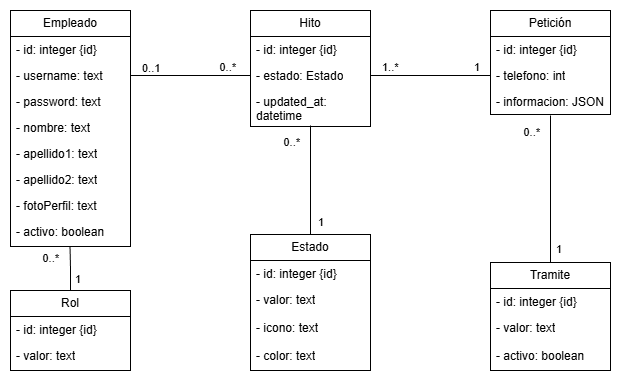
\includegraphics[width=1\textwidth]{img/diagramas/modelo_datos.png}
        \caption{Diagrama Entidad-Relación.}
        \label{fig:4.8}
    \end{figure}

\section{Diseño de la inteligencia artificial}
    El agente conversacional de Dialogflow funciona mediante la definición de intents y entities, implementando tecnologías de machine learning para detectar y analizar la intención que tiene el usuario. 
        
    Las posibles intenciones de los usarios se definen en los intents. 
    Se describen las frases de entrada o eventos que activan el intent, las contestaciones que debe dar el bot y las entities necesarias que se deben obtener. 
    Cuando el usuario dice una frase de entrada, la inteligencia artificial calcula la probabilidad de que coinicida con un intent, y si el porcentaje supera el umbral, activa la intención.
        
    Las entities sirven para definir los tipos de datos o la forma en la que se extrae la información de las frases.
    En otras palabras, sirven para categorizar o etiquetar las palabras. 
    Por ejemplo, "Quiero agendar una cita en la AEAT para mañana a las 10" podríamos extraer agendar una cita en la AEAT como una entidad de tipo trámite, mañana como fecha y las 10 como hora. 
    De esta forma también podemos saber que tipos de datos necesitamos al recopilar información, si un número, un texto, una dirección\dots
        
    Para la resolución de los trámites escogidos se han definido los siguientes intents: 
    \begin{itemize}
        \item Bienvenida: se activará automáticamente cuando el usuario inicia la llamada y activará un evento de espera de trámties.
        \item Tramite certificado empadronamiento, tramite cita AEAT y tramite tarjeta SACYL: se activarán cuando el usuario los solicite y el evento de espera de trámite esté activo y solicitarán los datos necesarios para cada trámite.
        \item Cita AEAT Modalidad: una vez recuperada la información inicial del tramite cita AEAT, se activa este intent desde el backend solo si el servicio escogido ofrece también cita telefónica.
        \item Cita AEAT Presencial: si el usuario solicita una cita presencial, el bot recupera la información correspondiente sobre la oficina y la fecha.
        \item Confirmar datos: una vez recuperada la información necesaria, se activará este intent para solicitar al usuario la vericidad de los datos y finalizar la llamada.
        \item Cambiar campo: en caso de que haya algún dato erróneo, se activará este intent para que el usuario pueda modificarlo.
    \end{itemize}

    También será necesario estipular los siguientes entities para facilitar la captura de la información: 
    \begin{itemize}
        \item Centros de salud de Valladolid: un enum con los centros de salud de Valladolid.
        \item DNI o pasaporte: una entidad regexp para limitar la variable al formato del DNI o pasaporte.
        \item Motivo tarjate SACYL: enum con los posibles motivos para solicitar la tarjeta.
        \item Municipios Valladolid: enum con todos los municipios de Valladolid.
        \item Oficina AEAT Valladolid: enum con las oficinas disponibles de la agencia tributaria en Valladolid.
        \item Servicios AEAT: un enum con la lista de servicios de la agencia tributaria.
        \item Teléfono: un variable regexp con el formato de los números telefónicos españoles.
        \item Tipo de cita: enum con los posibles tipos de cita en la AEAT.
        \item Trámite: enum con los trámites disponibles.
    \end{itemize}

    Por último, se ha definido en la figura \ref{fig:4.9} un digrama de flujo para definir la sescuencia prevista de una llamada al sistema.
    \begin{figure}[H]
        \centering
        
\includegraphics[width=0.8\textwidth]{img/diagramas/diagrama_flujo_ia.png}
        \caption{Diagrama de flujo del agente conversacional.}
        \label{fig:4.9}
    \end{figure}

\section{Seguridad y control de accesos}

\chapter{Implementación}
En este capítulo se resume el proceso de desarrollo del sistema elaborado, detallando los principales componentes que lo conforman y su funcionamiento. 
La explicación se estructura siguiendo el orden real de la implementación del proyecto, comenzando por el desarrollo del frontend, seguido de la creación de la base de datos y la construcción del backend. 
Finalmente, se comentan los distintos servicios integrados en la aplicación, como el envío de correos electrónicos, el bot de Discord, la conexión con la IA mediante Dialogflow y la automatización de los trámites con funciones de RPA. 

\section{Implementación del frontend}
    Para el desarrollo del frontend de la aplicación se ha utilizado el sistema de plantillas de Jinja. 
    Se ha definido una plantilla base (layout.jinja), mostrada en la figura \ref{fig:5.1}, que funciona como estructura común para todas las vistas de la web. 
    \begin{figure}[H]
        \centering
        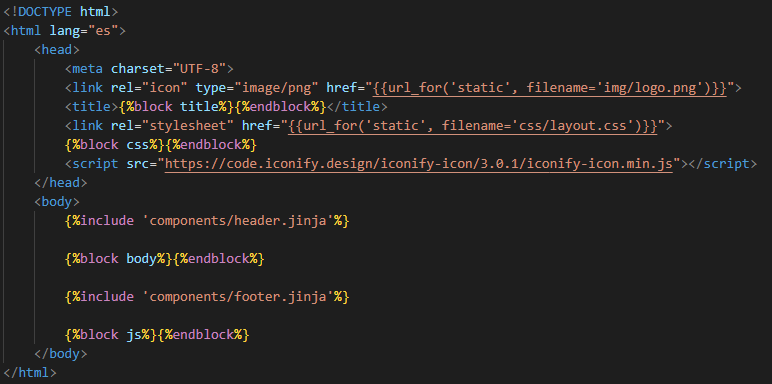
\includegraphics[width=0.75\textwidth]{img/desarrollo/layout.png}
        \caption{Código de la plantilla base layout.jinja.}
        \label{fig:5.1}
    \end{figure}
    Esta plantilla incluye componentes reutilizables del sistema, como la cabecera y el pie de página, permitiendo que el resto de vistas definan únicamente el contenido específico. 
    Este enfoque reduce la duplicación de código y mejora la mantenibilidad del sistema, facilitando las modificaciones globales.

    Asimismo, se importa una hoja de estilos CSS común para toda la aplicación, garantizando coherencia visual en todas las páginas mediante el uso de la misma paleta de colores, tipografía y estructura. 
    
    Por último, se integra la librería de iconos open source \href{https://iconify.design/}{Iconify} \cite{ref15}, lo que permite incorporar iconos de forma sencilla en las distintas vistas.

    Cabe destacar que el frontend incluye múltiples vistas con sus hojas de estilos y scripts dinámicos. 
    Sin embargo, en esta sección se comentan únicamente los elementos más representativos técnicamente, evitando detallar componentes HTML simples o repetitivos, o estilos o validaciones sin importancia. 

    \begin{figure}[H]
        \centering
        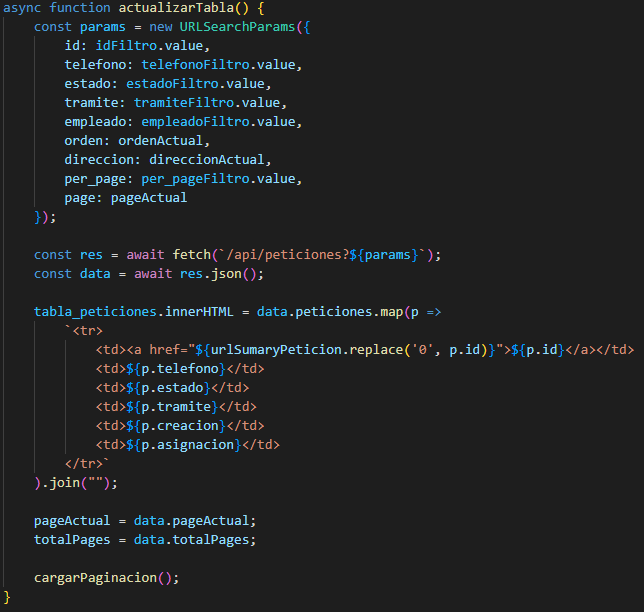
\includegraphics[width=0.75\textwidth]{img/desarrollo/peticionesjs.png}
        \caption{Fragmento de código de la construcción dinámica de la tabla de peticiones.}
        \label{fig:5.2}
    \end{figure}
    Los componentes principales de la web son las tablas que muestran la información correspondiente a las peticiones, empleados o trámites. 
    El contenido de estas tablas se carga dinámicamente en función de los los filtros, el orden o la paginación. 
    La figura \ref{fig:5.2} muestra el fragmento de código en el que se llama a un endpoint, "/api/peticiones", para recuperar la información correspondiente de la base de datos y actualizarla en la tabla.

    \begin{figure}[H]
        \centering
        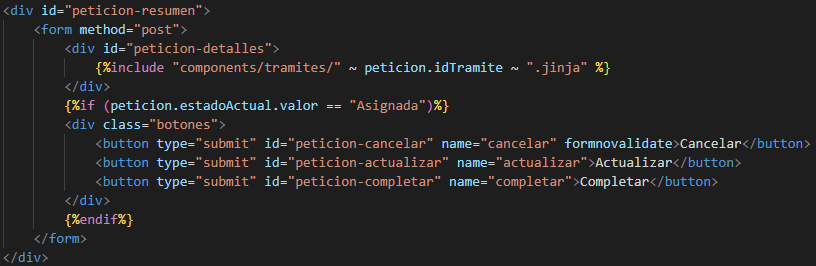
\includegraphics[width=0.75\textwidth]{img/desarrollo/sumaryPeticion.png}
        \caption{Fragmento de código de la plantilla resumen de una petición.}
        \label{fig:5.3}
    \end{figure}
    \begin{figure}[H]
        \centering
        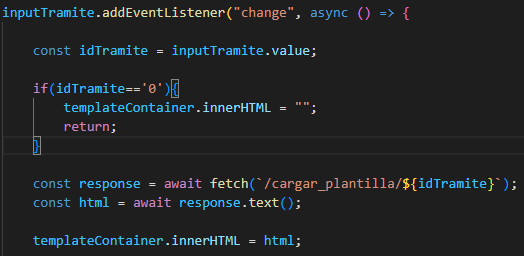
\includegraphics[width=0.6\textwidth]{img/desarrollo/crearPeticionjs.png}
        \caption{Fragmento de código de carga dinámica de las plantillas de cada trámite.}
        \label{fig:5.4}
    \end{figure}
    De forma análoga, las plantillas que contienen la información correspondiente a cada trámite se renderizan en tiempo de ejecución, mostrando el formulario correspondiente dependiendo del trámite escogido, figuras \ref{fig:5.3} y \ref{fig:5.4}. 

    El resto de componentes que abundan en la aplicación son formularios, que no presentan nada especial salvo alguna validación o evento dinámico.

\section{Implementación de la base de datos}
    La implementación de la base de datos se ha llevado a cabo mediante tablas SQL, definiendo en cada atributo su tipo de dato, restricciones de unicidad y posibilidad de valores nulos. 
    Asimismo, se han establecido las claves primarias para cada tabla y las claves foráneas para modelar las relaciones entre entidades.

    La figura \ref{fig:5.5} muestra la función encargada de inicializar la base de datos en la aplicación, ejecutando el archivo SQL correspondiente durante el arranque del sistema. 
    \begin{figure}[H]
        \centering
        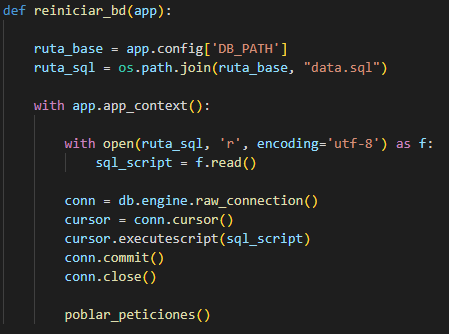
\includegraphics[width=0.6\textwidth]{img/desarrollo/utils_db.png}
        \caption{Código de la función de inicialización de la base de datos.}
        \label{fig:5.5}
    \end{figure}

    Para gestionar la base de datos dentro de la aplicación se utiliza SQLAlchemy, lo que permite definir clases Python equivalentes a cada tabla y trabajar con los registros como objetos. 
    La figura \ref{fig:5.6} muestra un ejemplo de consulta dinámica sobre la tabla de peticiones, en la que se aplican filtros, ordenación y paginación en función de los parámetros recibidos. 
    El resultado se almacena en la variable "peticiones" como una lista de objetos de la clase correspondiente, permitiendo acceder a sus atributos y métodos directamente.
    \begin{figure}[H]
        \centering
        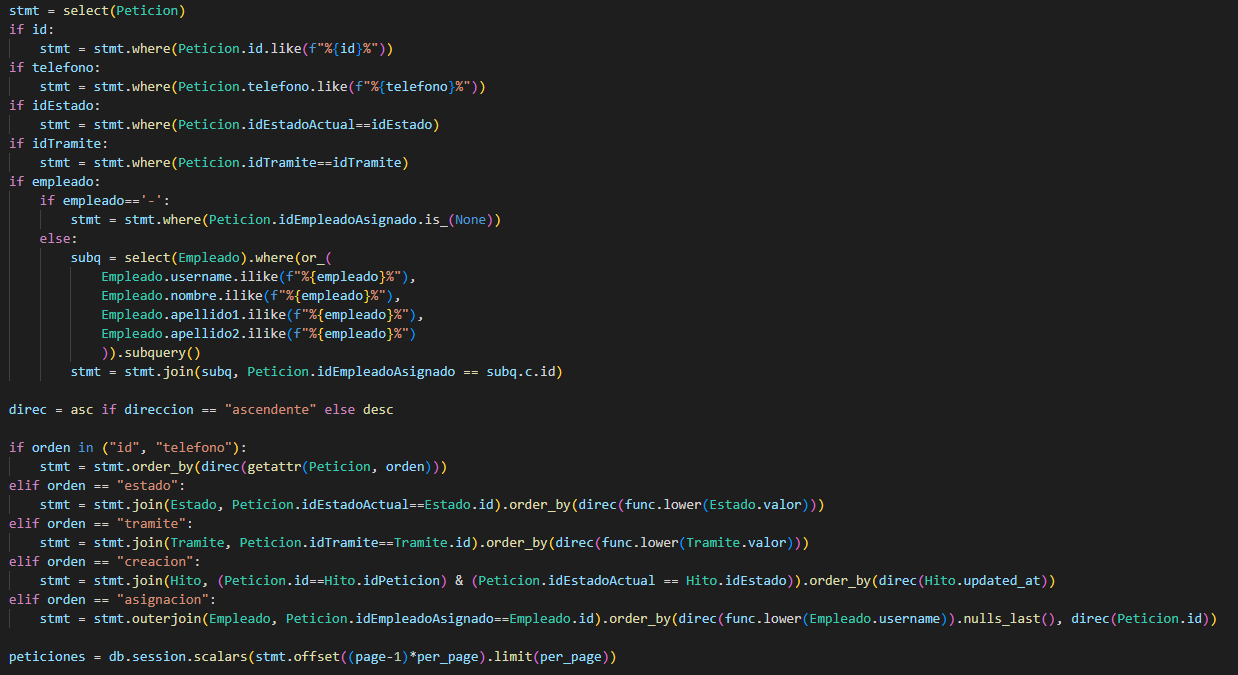
\includegraphics[width=1\textwidth]{img/desarrollo/dashboard.png}
        \caption{Fragmento de código de la consulta de peticiones.}
        \label{fig:5.6}
    \end{figure}

\section{Implementación del backend}
    En esta sección se va a tratar el desarrollo del backend de la aplicación web, centrándolo en las rutas que ejercen como controladores de las vistas. 
    Por modularidad, se han definido distintos blueprints para cada parte de la aplicación, permitiendo organizar el código de forma más clara dividiendo las rutas y su lógica en distintos archivos Python. 
    
    El primer blueprint es el de inicio, que se encarga de redireccionar al inicio de sesión. 
    También incluye un endpoint que renderiza la plantilla con la información de cada trámite, llamado dinámicamente desde el formulario de crear peticiones. 

    El segundo blueprint es el de autenticación, que incluye las rutas para iniciar y cerrar sesión. 
    Las sesiones se gestionan mediante la extensión Flask-Login, que incluye funciones que simplifican la gestión de usuarios identidficados, como el decorador @login\_required, que se escribe en las funciones de las rutas para bloquear el acceso a usuarios no autenticados. 
    Además, se ha implementado un sistema de permisos para cada rol, figura \ref{fig:5.7}, que se almacenan en un archivo JSON y se cargan en la sesión de cada usuario cuando se identifican. 
    La figura \ref{fig:5.8} muestra el código de las funciones que gestionan los permisos, incluido un decorador personalizado, @permiso\_requerido, que actua de forma análoga a @login\_required, bloqueando el acceso a las rutas a las que el usuario no tenga permiso.
    \begin{figure}[H]
        \centering
        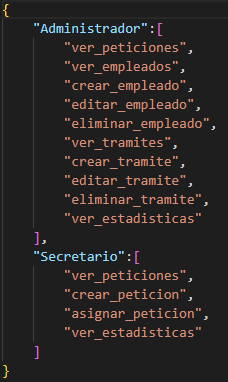
\includegraphics[width=0.2\textwidth]{img/desarrollo/permisosjson.png}
        \caption{JSON con los permisos de cada rol.}
        \label{fig:5.7}
    \end{figure}
    \begin{figure}[H]
        \centering
        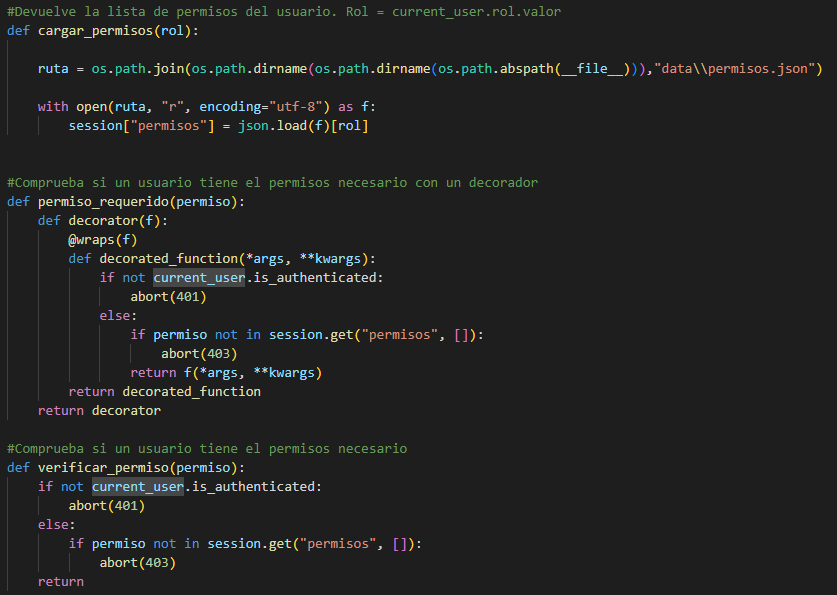
\includegraphics[width=0.7\textwidth]{img/desarrollo/permisospy.png}
        \caption{Código de las funciones para la gestión de permisos en la aplicación.}
        \label{fig:5.8}
    \end{figure}

    El tercer blueprint es el más importante, incluye las rutas que gestionan las vistas y funcionalidades principales de la aplicación. 
    En este módulo se encuentran las funciones que gestionan las peticiones, empleados, trámites y la información del perfil de cada empleado. 
    Estas funciones incluyen principalmente la lógica para recuperar la información necesaria de la base de datos, como en la figura \ref{fig:5.6}, renderizar las plantillas correspondientes y gestionar la información recibida de los formularios. 
    
    Tanto las peticiones como los empleados y trámites se gestionan de forma similar en el backend, ya que comparten la forma en la que se presentan en el frontend.
    En los tres casos se ha implementado una ruta para renderizar la página con la tabla y un endpoint para recuperar la información de la tabla en formato JSON. 
    En el supuesto de las peticiones se ha añadido una ruta para mostrar el resumen de cada petición, con la funcionalidad correspondiente para asignarse la petición, completarla, cancelarla, editarla o desasignársela, y otra ruta independiente para crear nuevas peticiones.
    Sin embargo, en el caso de los empleados y trámites se simplifica la lógica reutilizando la misma ruta y plantilla tanto para mostrar los datos individuales y editarlos como para crear nuevos registros, diferenciando ambos casos mediante la presencia o ausencia de un ID en la URL.

    El cuarto blueprint sirve para gestionar la carga y subida de archivos en la web. 
    Hasta el momento, esta funcionalidad se utiliza únicamente para recuperar la imagen de perfil de cada empleado que se muestra tanto en el perfil como en el historial de cada petición. 
    También permite modificar la imagen de perfil, almacenando la imagen nueva y borrando la antigua. 

    Por último, hay un blueprint de errores, que se encarga únicamente de renderizar una plantilla personalizada en caso de error 404, es decir, cuando el empleado intenta acceder a un recurso inexistente, y de error 403, cuando el empleado intenta acceder a un recurso para el que no tiene permiso.
    
    Adicionalmente, se ha implementado otro blueprint independiente para modularizar la lógica de las APIs 
    Por el momento, este incluye un único endpoint que actúa como webhook para procesar los eventos de Dialogflow, cuya integración se comentará con mayor detalle en la sección siguiente.

\section{Implementación e integración de servicios}
    Esta sección se centra en explicar la implementación de los cuatro servicios integrados en la aplicación, poniendo especial atención en aquellos relacionados con la gestión de las llamadas, ya que constituyen el eje central del proyecto. 
    
    \subsection{Implementación e integración del servicio de correo electrónico}
        Para la gestión del envío de correos electrónicos dentro de la aplicación web se ha utilizado la extensión Flask-Mail, que permite integrar facilmente un sistema de notificaciones por correo electrónico dentro del framework Flask. 
        Este servicio se utiliza para comunicar automáticamente a los empleado distinta información relacionada con su cuenta, como el envío de sus credenciales de acceso, el establecimiento de una nueva contraseña temporal o la activación y desactivación del acceso al sistema. 

        Teniendo en cuenta el alcance del proyecto, no se ha configurado un servidor de correo real. 
        En su lugar, se ha utilizado un servidor SMTP local de pruebas ejecutado en localhost mediante la herramienta aiosmtpd. 
        De esta forma, los correos generados por la aplicación se muestran por consola, lo que permite verificar su correcto funcionamiento sin necesidad de utilizar un servidor real. 

        Finalmente, la configuración actual del servicio de correo electrónico se encuentra en el archivo config.py, donde se definen los parámetro necesarios para su funcionamiento, siendo fácilmente modificable para la futura integración del servidor real que se utilice en producción. 
        El envío de correos se realiza de forma centralizada mediante una única función, figura \ref{fig:5.9}, lo que permite generar distintos tipos de mensajes ajustando únicamente los parámetros de entrada. 
        \begin{figure}[H]
            \centering
            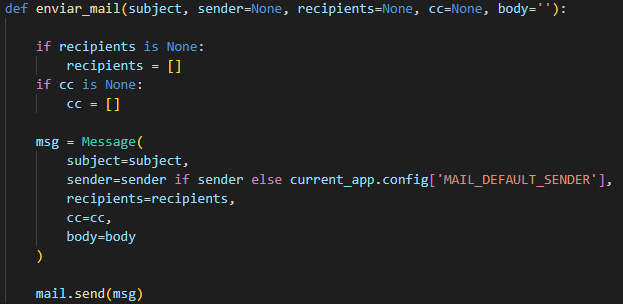
\includegraphics[width=0.5\textwidth]{img/desarrollo/mailpy.png}
            \caption{Código de la función de envío de correos electrónicos.}
            \label{fig:5.9}
        \end{figure}

    \subsection{Implementación e integración del bot de Discord}
        

\chapter{Pruebas}
Con el objetivo de validar el correcto funcionamiento del sistema implementado, se han realizado una serie de pruebas funcionales manuales sobre los distintos módulos que componen el proyecto. 
Aunque durante el desarrollo se llevaron a cabo verificaciones parciales para comprobar el progreso y corregir errores, las pruebas descritas en este capítulo se realizaron con el desarrollo finalizado. 

Las pruebas se han realizado en un entorno local de desarrollo, utilizando el navegador Google Chrome para el acceso a la aplicación web y la aplicación de escritorio de Discord como medio de comunicación por voz con el sistema. 
Se ha empleado la versión de escritorio de Discord para garantizar una mayor estabilidad en la transmisión de audio, ya que la versión móvil presenta una conexión más inestable que puede acarrear en pérdidas puntuales de paquetes. 


\subsection{Pruebas del sistema web}

    \begin{table}[H]
        \centering
        \begin{tabular}{|l|p{12cm}|}
        \hline
        \textbf{WEB01} & Inicio de sesión exitoso. \\ \hline
        \textbf{Descripción} & El empleado se identifica en la plataforma web con sus credenciales. \\ \hline
        \textbf{Resultado esperado} & Se redirige a la página de inicio, con el empleado identificado en el sistema y con los permisos correspondientes cargados en la sesión. \\ \hline
        \textbf{Resultado obtenido} &  \\ \hline
        \end{tabular}
        \caption{Caso de prueba WEB01 - Inicio de sesión exitoso}
    \end{table}

    \begin{table}[H]
        \centering
        \begin{tabular}{|l|p{12cm}|}
        \hline
        \textbf{WEB02} & Inicio de sesión denegado. \\ \hline
        \textbf{Descripción} & El empleado introduce sus credenciales en la plataforma web con su cuenta desactivada. \\ \hline
        \textbf{Resultado esperado} & El sistema deniega el inicio de sesión y avisa al empleado que su cuenta está desactivada. \\ \hline
        \textbf{Resultado obtenido} &  \\ \hline
        \end{tabular}
        \caption{Caso de prueba WEB02 - Inicio de sesión denegado}
    \end{table}

    \begin{table}[H]
        \centering
        \begin{tabular}{|l|p{12cm}|}
        \hline
        \textbf{WEB03} & Buscar una petición. \\ \hline
        \textbf{Descripción} & El empleado busca una petición en la tabla de peticiones mediante los filtros. \\ \hline
        \textbf{Resultado esperado} & La tabla muestra las peticiones coincidentes con los criterios de búsqueda. \\ \hline
        \textbf{Resultado obtenido} &  \\ \hline
        \end{tabular}
        \caption{Caso de prueba WEB03 - Buscar una petición}
    \end{table}

    \begin{table}[H]
        \centering
        \begin{tabular}{|l|p{12cm}|}
        \hline
        \textbf{WEB04} & Crear una petición manualmente. \\ \hline
        \textbf{Descripción} &  Un secretario crea una petición rellenando un formulario manualmente desde la plataforma web. \\ \hline
        \textbf{Resultado esperado} & Se genera una nueva petición en el sistema con los datos introducidos. \\ \hline
        \textbf{Resultado obtenido} &  \\ \hline
        \end{tabular}
        \caption{Caso de prueba WEB04 - Crear una petición manualmente}
    \end{table}

    \begin{table}[H]
        \centering
        \begin{tabular}{|l|p{12cm}|}
        \hline
        \textbf{WEB05} & Asignarse una petición. \\ \hline
        \textbf{Descripción} & Un secretario se asigna una petición cuyo estado es pendiente. \\ \hline
        \textbf{Resultado esperado} & Se actualiza el estado de la petición a asignada y se muestra el menú de edición de la petición al empleado asignado. \\ \hline
        \textbf{Resultado obtenido} &  \\ \hline
        \end{tabular}
        \caption{Caso de prueba WEB05 - Asignarse una petición}
    \end{table}

    \begin{table}[H]
        \centering
        \begin{tabular}{|l|p{12cm}|}
        \hline
        \textbf{WEB06} & Desasignarse una petición. \\ \hline
        \textbf{Descripción} & Un secretario se desasigna un petición que tenía asignada. \\ \hline
        \textbf{Resultado esperado} & Se actualiza el estado de la petición a pendiente y se oculta el menú de edición de la petición al empleado. \\ \hline
        \textbf{Resultado obtenido} &  \\ \hline
        \end{tabular}
        \caption{Caso de prueba WEB06 - Desasignarse una petición}
    \end{table}

    \begin{table}[H]
        \centering
        \begin{tabular}{|l|p{12cm}|}
        \hline
        \textbf{WEB07} & Editar los datos de una petición. \\ \hline
        \textbf{Descripción} & El secretario asignado a una petición modifica su información y la guarda. \\ \hline
        \textbf{Resultado esperado} & Se actualiza la información de la petición en la base de datos. \\ \hline
        \textbf{Resultado obtenido} &  \\ \hline
        \end{tabular}
        \caption{Caso de prueba WEB07 - Editar los datos de una petición}
    \end{table}

    \begin{table}[H]
        \centering
        \begin{tabular}{|l|p{12cm}|}
        \hline
        \textbf{WEB08} & Cancelar una petición. \\ \hline
        \textbf{Descripción} & El secretario asignado a una petición la cancela. \\ \hline
        \textbf{Resultado esperado} & Se actualiza el estado de la petición a cancelada y no se completa el trámite. \\ \hline
        \textbf{Resultado obtenido} &  \\ \hline
        \end{tabular}
        \caption{Caso de prueba WEB08 - Cancelar una petición}
    \end{table}

    \begin{table}[H]
        \centering
        \begin{tabular}{|l|p{12cm}|}
        \hline
        \textbf{WEB09} & Completar una petición de certificado de empadronamiento. \\ \hline
        \textbf{Descripción} & El secretario asignado a una petición de certificado de empadronamiento la completa. \\ \hline
        \textbf{Resultado esperado} & Se abre un navegador en la página del Ayuntamiento de Valladolid donde se completa el trámite del certificado de empadronamiento, se rellena el formulario automáticamente con la información de la petición y se actualiza el estado de la petición a completada. \\ \hline
        \textbf{Resultado obtenido} &  \\ \hline
        \end{tabular}
        \caption{Caso de prueba WEB09 - Completar una petición de certificado de empadronamiento}
    \end{table}

    \begin{table}[H]
        \centering
        \begin{tabular}{|l|p{12cm}|}
        \hline
        \textbf{WEB10} & Completar una petición de cita en la AEAT. \\ \hline
        \textbf{Descripción} & El secretario asignado a una petición de cita en la AEAT la completa. \\ \hline
        \textbf{Resultado esperado} & Se abre un navegador en la página de citas de la Agencia Tributaria, se completan los menús y formularios automáticamente con la información de la petición y se actualiza el estado de la petición a completada. \\ \hline
        \textbf{Resultado obtenido} &  \\ \hline
        \end{tabular}
        \caption{Caso de prueba WEB10 - Completar una petición de cita en la AEAT}
    \end{table}

    \begin{table}[H]
        \centering
        \begin{tabular}{|l|p{12cm}|}
        \hline
        \textbf{WEB11} & Completar una petición de tarjeta de SACYL. \\ \hline
        \textbf{Descripción} & El secretario asignado a una petición de tarjeta sanitaria la completa. \\ \hline
        \textbf{Resultado esperado} & Se abre un navegador en la página de SACYL donde se solicita la tarjeta sanitaria, se rellena el formulario automáticamente con la información de la petición y se actualiza el estado de la petición a completada. \\ \hline
        \textbf{Resultado obtenido} &  \\ \hline
        \end{tabular}
        \caption{Caso de prueba WEB11 - Completar una petición de tarjeta de SACYL}
    \end{table}

    \begin{table}[H]
        \centering
        \begin{tabular}{|l|p{12cm}|}
        \hline
        \textbf{WEB12} & Buscar un empleado. \\ \hline
        \textbf{Descripción} & Un administrados busca un empleado en la tabla de empleados mediante los filtros. \\ \hline
        \textbf{Resultado esperado} & La tabla muestra los empleados coincidentes con los criterios de búsqueda. \\ \hline
        \textbf{Resultado obtenido} &  \\ \hline
        \end{tabular}
        \caption{Caso de prueba WEB12 - Buscar un empleado}
    \end{table}

    \begin{table}[H]
        \centering
        \begin{tabular}{|l|p{12cm}|}
        \hline
        \textbf{WEB13} & Crear un empleado. \\ \hline
        \textbf{Descripción} & Un administrador crea una cuenta de empleado rellenando un formulario en la plataforma web. \\ \hline
        \textbf{Resultado esperado} & Se genera una nueva cuenta de empleado en el sistema con los datos introducidos, comprobando que no exista otra cuenta con el mismo correo, y se envía un email a la cuenta creada con su usuario y su contraseña temporal. \\ \hline
        \textbf{Resultado obtenido} &  \\ \hline
        \end{tabular}
        \caption{Caso de prueba WEB13 - Crear un empleado}
    \end{table}

    \begin{table}[H]
        \centering
        \begin{tabular}{|l|p{12cm}|}
        \hline
        \textbf{WEB14} & Modificar información de un empleado. \\ \hline
        \textbf{Descripción} & Un administrador modifica la información de un empleado y la guarda. \\ \hline
        \textbf{Resultado esperado} & El sistema actualiza la información de la cuenta y si se ha modificado el correo comprueba que no haya otra cuenta con el mismo. \\ \hline
        \textbf{Resultado obtenido} &  \\ \hline
        \end{tabular}
        \caption{Caso de prueba WEB14 - Modificar información de un empleado}
    \end{table}

    \begin{table}[H]
        \centering
        \begin{tabular}{|l|p{12cm}|}
        \hline
        \textbf{WEB15} & Desactivar una cuenta de empleado. \\ \hline
        \textbf{Descripción} & Un administrador desactiva la cuenta de un empleado. \\ \hline
        \textbf{Resultado esperado} & Se deniega el acceso de la cuenta al sistema, se desasignan todas las peticiones asignadas por este empleado camnbiando el estado a pendiente y se notifica por correo al empleado que su cuenta ha sido desactivada. \\ \hline
        \textbf{Resultado obtenido} &  \\ \hline
        \end{tabular}
        \caption{Caso de prueba WEB15 - Desactivar una cuenta de empleado}
    \end{table}

    \begin{table}[H]
        \centering
        \begin{tabular}{|l|p{12cm}|}
        \hline
        \textbf{WEB16} & Activar una cuenta de empleado. \\ \hline
        \textbf{Descripción} & Un administrador activa la cuenta de un empleado. \\ \hline
        \textbf{Resultado esperado} & Se permite el acceso de la cuenta al sistema y se notifica por correo al empleado que su cuenta ha sido reactivada. \\ \hline
        \textbf{Resultado obtenido} &  \\ \hline
        \end{tabular}
        \caption{Caso de prueba WEB16 - Activar una cuenta de empleado}
    \end{table}

    \begin{table}[H]
        \centering
        \begin{tabular}{|l|p{12cm}|}
        \hline
        \textbf{WEB17} & Reestablecer contraseña de un empleado. \\ \hline
        \textbf{Descripción} & Un administrador restablece la contraseña de un empleado. \\ \hline
        \textbf{Resultado esperado} & Se modifica la contraseña del empleado a una contraseña temporal generada automáticamente y se envía la contraseña por correo al empleado.  \\ \hline
        \textbf{Resultado obtenido} &  \\ \hline
        \end{tabular}
        \caption{Caso de prueba WEB17 - Reestablecer contraseña de un empleado}
    \end{table}

    \begin{table}[H]
        \centering
        \begin{tabular}{|l|p{12cm}|}
        \hline
        \textbf{WEB18} & Buscar un trámite. \\ \hline
        \textbf{Descripción} & Un administrados busca un trámite en la tabla de trámites mediante los filtros. \\ \hline
        \textbf{Resultado esperado} & La tabla muestra los trámites coincidentes con los criterios de búsqueda. \\ \hline
        \textbf{Resultado obtenido} &  \\ \hline
        \end{tabular}
        \caption{Caso de prueba WEB18 - Buscar un trámite}
    \end{table}

    \begin{table}[H]
        \centering
        \begin{tabular}{|l|p{12cm}|}
        \hline
        \textbf{WEB19} & Crear un trámite. \\ \hline
        \textbf{Descripción} & Un administrador genera un nuevo trámite rellenando un formulario. \\ \hline
        \textbf{Resultado esperado} & Se genera un nuevo trámite en el sistema, comprobando que no existe otro trámite con el mismo título. \\ \hline
        \textbf{Resultado obtenido} &  \\ \hline
        \end{tabular}
        \caption{Caso de prueba WEB19 - Crear un trámite}
    \end{table}

    \begin{table}[H]
        \centering
        \begin{tabular}{|l|p{12cm}|}
        \hline
        \textbf{WEB20} & Modificar el título de un trámite. \\ \hline
        \textbf{Descripción} & Un administrador edita la información de un trámite. \\ \hline
        \textbf{Resultado esperado} & Se actualiza la información del trámite en el sistema, comprobando que no existe ningún otro trámite con el mismo título en caso de que se haya modificado. \\ \hline
        \textbf{Resultado obtenido} &  \\ \hline
        \end{tabular}
        \caption{Caso de prueba WEB20 - Modificar el título de un trámite}
    \end{table}

    \begin{table}[H]
        \centering
        \begin{tabular}{|l|p{12cm}|}
        \hline
        \textbf{WEB21} & Desactivar un trámite. \\ \hline
        \textbf{Descripción} & Un administrador desactiva un trámite activo. \\ \hline
        \textbf{Resultado esperado} & Se cancelan automáticamente todas las peticiones no finalizadas de ese trámite y no deja crear nuevas peticiones para esta gestión. \\ \hline
        \textbf{Resultado obtenido} &  \\ \hline
        \end{tabular}
        \caption{Caso de prueba WEB21 - Desactivar un trámite}
    \end{table}

    \begin{table}[H]
        \centering
        \begin{tabular}{|l|p{12cm}|}
        \hline
        \textbf{WEB22} & Activar un trámite. \\ \hline
        \textbf{Descripción} & Un administrador activa un trámite desactivado. \\ \hline
        \textbf{Resultado esperado} & Se permite la creación de nuevas peticiones para esta gestión. \\ \hline
        \textbf{Resultado obtenido} &  \\ \hline
        \end{tabular}
        \caption{Caso de prueba WEB22 - Activar un trámite}
    \end{table}

    \begin{table}[H]
        \centering
        \begin{tabular}{|l|p{12cm}|}
        \hline
        \textbf{WEB23} & Cambiar la foto de perfil. \\ \hline
        \textbf{Descripción} & Un empleado modifica la foto de perfil de su cuenta. \\ \hline
        \textbf{Resultado esperado} & Se borra la foto de perfil antigua para almacena la nueva en su lugar, refrescando la web para mostrar la foto nueva.  \\ \hline
        \textbf{Resultado obtenido} &  \\ \hline
        \end{tabular}
        \caption{Caso de prueba WEB23 - Cambiar la foto de perfil}
    \end{table}

    \begin{table}[H]
        \centering
        \begin{tabular}{|l|p{12cm}|}
        \hline
        \textbf{WEB24} & Cambiar la contraseña de la cuenta. \\ \hline
        \textbf{Descripción} & Un empleado modifica la contraseña de su cuenta introduciendo la contraseña antigua y la nueva. \\ \hline
        \textbf{Resultado esperado} & Se comprueba que la contraseña antigua es correcta y se actualiza la contraseña de la cuenta con la nueva.  \\ \hline
        \textbf{Resultado obtenido} &  \\ \hline
        \end{tabular}
        \caption{Caso de prueba WEB24 - Cambiar la contraseña de la cuenta}
    \end{table}


\subsection{Pruebas del agente conversacional}

    \begin{table}[H]
        \centering
        \begin{tabular}{|l|p{12cm}|}
        \hline
        \textbf{AC01} & Detección del trámite \\ \hline
        \textbf{Descripción} &  \\ \hline
        \textbf{Resultado esperado} &  \\ \hline
        \textbf{Resultado obtenido} &  \\ \hline
        \end{tabular}
        \caption{Caso de prueba AC01 - }
    \end{table}

    \begin{table}[H]
        \centering
        \begin{tabular}{|l|p{12cm}|}
        \hline
        \textbf{AC02} & Extracción de datos para el certificado de empadronamiento. \\ \hline
        \textbf{Descripción} &  \\ \hline
        \textbf{Resultado esperado} &  \\ \hline
        \textbf{Resultado obtenido} &  \\ \hline
        \end{tabular}
        \caption{Caso de prueba AC02 - }
    \end{table}

    \begin{table}[H]
        \centering
        \begin{tabular}{|l|p{12cm}|}
        \hline
        \textbf{AC03} & Extracción de datos para la cita de la AEAT. \\ \hline
        \textbf{Descripción} &  \\ \hline
        \textbf{Resultado esperado} &  \\ \hline
        \textbf{Resultado obtenido} &  \\ \hline
        \end{tabular}
        \caption{Caso de prueba AC03 - }
    \end{table}

    \begin{table}[H]
        \centering
        \begin{tabular}{|l|p{12cm}|}
        \hline
        \textbf{AC04} & Extracción de datos para la tarjeta de SACYL. \\ \hline
        \textbf{Descripción} &  \\ \hline
        \textbf{Resultado esperado} &  \\ \hline
        \textbf{Resultado obtenido} &  \\ \hline
        \end{tabular}
        \caption{Caso de prueba AC04 - }
    \end{table}

    \begin{table}[H]
        \centering
        \begin{tabular}{|l|p{12cm}|}
        \hline
        \textbf{AC05} & Modificar uno de los datos extraídos. \\ \hline
        \textbf{Descripción} &  \\ \hline
        \textbf{Resultado esperado} &  \\ \hline
        \textbf{Resultado obtenido} &  \\ \hline
        \end{tabular}
        \caption{Caso de prueba AC05 - }
    \end{table}

    \begin{table}[H]
        \centering
        \begin{tabular}{|l|p{12cm}|}
        \hline
        \textbf{AC06} & Responder preguntas sin perder el flujo. \\ \hline
        \textbf{Descripción} &  \\ \hline
        \textbf{Resultado esperado} &  \\ \hline
        \textbf{Resultado obtenido} &  \\ \hline
        \end{tabular}
        \caption{Caso de prueba AC06 - }
    \end{table}

    \begin{table}[H]
        \centering
        \begin{tabular}{|l|p{12cm}|}
        \hline
        \textbf{AC07} & Intención del usuario no reconocida. \\ \hline
        \textbf{Descripción} &  \\ \hline
        \textbf{Resultado esperado} &  \\ \hline
        \textbf{Resultado obtenido} &  \\ \hline
        \end{tabular}
        \caption{Caso de prueba AC07 - }
    \end{table}

\subsection{Pruebas del bot de Discord}

    \begin{table}[H]
        \centering
        \begin{tabular}{|l|p{12cm}|}
        \hline
        \textbf{DISC01} & Conexión al canal de voz. \\ \hline
        \textbf{Descripción} &  \\ \hline
        \textbf{Resultado esperado} &  \\ \hline
        \textbf{Resultado obtenido} &  \\ \hline
        \end{tabular}
        \caption{Caso de prueba DISC01 - }
    \end{table}

    \begin{table}[H]
        \centering
        \begin{tabular}{|l|p{12cm}|}
        \hline
        \textbf{DISC02} & Recepción de audio del canal de voz. \\ \hline
        \textbf{Descripción} &  \\ \hline
        \textbf{Resultado esperado} &  \\ \hline
        \textbf{Resultado obtenido} &  \\ \hline
        \end{tabular}
        \caption{Caso de prueba DISC02 - }
    \end{table}

    \begin{table}[H]
        \centering
        \begin{tabular}{|l|p{12cm}|}
        \hline
        \textbf{DISC03} & Reproducción de audio en el canal de voz. \\ \hline
        \textbf{Descripción} &  \\ \hline
        \textbf{Resultado esperado} &  \\ \hline
        \textbf{Resultado obtenido} &  \\ \hline
        \end{tabular}
        \caption{Caso de prueba DISC03 - }
    \end{table}

    \begin{table}[H]
        \centering
        \begin{tabular}{|l|p{12cm}|}
        \hline
        \textbf{DISC04} & Colgar la llamada. \\ \hline
        \textbf{Descripción} &  \\ \hline
        \textbf{Resultado esperado} &  \\ \hline
        \textbf{Resultado obtenido} &  \\ \hline
        \end{tabular}
        \caption{Caso de prueba DISC04 - }
    \end{table}


\subsection{Pruebas de integración}

    \begin{table}[H]
        \centering
        \begin{tabular}{|l|p{12cm}|}
        \hline
        \textbf{INT01} & Solicitud completa del certificado de empadronamiento. \\ \hline
        \textbf{Descripción} &  \\ \hline
        \textbf{Resultado esperado} &  \\ \hline
        \textbf{Resultado obtenido} &  \\ \hline
        \end{tabular}
        \caption{Caso de prueba INT01 - }
    \end{table}

    \begin{table}[H]
        \centering
        \begin{tabular}{|l|p{12cm}|}
        \hline
        \textbf{INT02} & Solicitud completa de la cita en la AEAT. \\ \hline
        \textbf{Descripción} &  \\ \hline
        \textbf{Resultado esperado} &  \\ \hline
        \textbf{Resultado obtenido} &  \\ \hline
        \end{tabular}
        \caption{Caso de prueba INT02 - }
    \end{table}

    \begin{table}[H]
        \centering
        \begin{tabular}{|l|p{12cm}|}
        \hline
        \textbf{INT03} & Solicitud completa de la tarjeta de SACYL. \\ \hline
        \textbf{Descripción} &  \\ \hline
        \textbf{Resultado esperado} &  \\ \hline
        \textbf{Resultado obtenido} &  \\ \hline
        \end{tabular}
        \caption{Caso de prueba INT03 - }
    \end{table}

\chapter{Conclusiones y trabajo futuro}
\section{Conclusiones}

    % \subsection{Dificultades observadas}
    %     %TODO ACABAR
    %     1. Coste de las tecnologías: 
    %     2. Autentificación frente el sistema: surge
    %     una necesidad en la producción futura del sistema y es la forma de
    %     identificar al llamante. Esto es necesario para distintos trámites, en
    %     cuestión de protección de datos y para evitar estafas. Para la simulación
    %     actual no es del todo necesario, ya que es un entorno controlado, pero nos
    %     reduce mucho el número de trámites que puedo elegir, ya que la mayoría no
    %     están pensados a hacerlos por terceros y requieren de identificación
    %     mediante DNI electrónico o certificado digital.

\section{Trabajo futuro}
%NOTE Mejoras en la app: gestión de trámites para que administradores añadan, modifiquen, eliminen tramites.




%Esto es una cita: \cite{ej}. Tiene que hacer referencia a la etiqueta de un bibitem.

%Esto es un enlace \href{www.enlace.net}{Enlace}

% Esto es una url \url{http://www.uva.es}


\cleardoublepage

%\nocite{*}
\bibliographystyle{ieeetr}
% La bibliografía se detalla en el archivo bibliografia.bib
\bookmarksetup{startatroot}
\bibliography{bibliografia}
\addcontentsline{toc}{chapter}{Bibliografía}

\appendix

\chapter{Manuales}\label{aped.A}
\section{Manual de instalación y despliegue} 

    \subsection{Dependencias del sistema}
        El sistema desarrollado depende de varios servicios externos que permiten el funcionamiento del agente conversacional y la comunicación entre los distintos componentes del sistema. 
        Concretamente, el sistema requiere el uso de los siguientes servicios: 
        \begin{itemize}
            \item Discord, utilizado para realizar las llamadas VoIP, capturando y reproduciendo audio de un canal de voz.
            \item Dialogflow, encargado de interpretar la intención del usuario y recopilar la información necesaria para realizar el trámite. 
            \item Google Cloud, necesario para la comunicación entre el bot de Discord y Dialogflow y el uso del servicio de reconocimiento de voz.  
            \item Ngrok, utilizado para exponer el servidor local de desarrollo a Internet, permitiendo la comunicación entre Dialogflow y la plataforma web.
        \end{itemize}
        
        Además, para ejecutar el sistema es necesario disponer del siguiente software: 
        \begin{itemize}
            \item Python 3.13 o superior.
            \item Gestor de paquetes pip.
            \item Navegador web moderno.
            \item Cuenta en Ngrok.
            \item Cuenta en Google Cloud.
            \item Cuenta en Discord.
        \end{itemize}

        Todas las dependencias necesarias para ejecutar el sistema se encuentran definidas en el archivo \textbf{requirements.txt}.

    \subsection{Instalación del proyecto}
        Para instalar el proyecto es necesario clonar el repositorio y preparar el entorno de ejecución de Python. 

        En primer lugar, se debe clonar el repositorio mediante el comando \textbf{git clone \url{https://github.com/humaral/tfg.git}}.
        
        Una vez descargado, se accede al directorio del repositorio con \textbf{cd tfg}. 
        
        Posteriormente, se crea un entorno virtual de Python para aislar las dependencias del proyecto con \textbf{python -m venv venv}.

        Una vez creado el entorno virtual, se activa con \textbf{venv\textbackslash{}Scripts\textbackslash{}activate} en sistemas Windows, y con \textbf{source venv/bin/activate} en Linux o MacOS. 

        Finalmente, se intalan las dependencias necesarias para ejecutar el proyecto con \textbf{pip install -r requirements.txt}.

        Además, es necesario crear un archivo \textbf{.env} que contenga las variables de entorno utilizadas por la aplicación. 
        Debe incluir al menos las siguientes variables:
        \begin{itemize}
            \item \textbf{DIALOGFLOW\_CREDENTIALS}
            \item \textbf{DISCORD\_TOKEN}
            \item \textit{VOSK\_MODEL\_PATH} (\textit{opcional}).
        \end{itemize}

    \subsection{Configuración del agente de Dialogflow}

        El repositorio incluye una copia exportada del agente conversacional utilizado por el sistema, ubicada en \textbf{/scripts\_aux/services/models/Operador.zip}.
        Pasos para importar este agente en Dialogflow se deben seguir los siguientes pasos:
        \begin{enumerate}
            \item Acceder a la \href{https://dialogflow.cloud.google.com}{consola de Dialogflow} - \url{https://dialogflow.cloud.google.com}.
            \item Crear un nuevo agente.
            \item Seleccionar la opción \textbf{Import from ZIP} en la configuración.
            \item Subir el archivo \textbf{Operador.zip}.
        \end{enumerate}

    \subsection{Configuración de Google Cloud}

        Para que la aplicación pueda comunicarse con Dialogflow y para poder usar los servicios de STT es necesario disponer de credenciales de Google Cloud. 
        La configuración de este servicio se consigue siguiendo los siguientes pasos:
        \begin{enumerate}
            \item Acceder a la \href{https://console.cloud.google.com/}{consola de Google Cloud} - \url{https://console.cloud.google.com/}.
            \item Crear un proyecto de Google Cloud.
            \item Activar el servicio de facturación.
            \item Vincular el agente de Dialogflow al proyecto.
            \item Activar el servicio de Speech-to-Text en el proyecto. (\textit{opcional})
            \item Crear una \textbf{Cloud Resource Manager API} asociada a los servicios de Dialogflow y STT y descargar el archivo JSON con sus credenciales.
            \item Añadir en el archivo \textbf{.env} la variable de entorno \textbf{DIALOGFLOW\_CREDENTIALS} con la ruta donde se almacene el archivo JSON con las credenciales.
        \end{enumerate}

    \subsection{Configuración de Vosk}

        En caso de preferir usar un modelo local para realizar el Speech-to-Text en vez del servicio de Google, se puede conseguir siguiendo estos pasos:
        \begin{enumerate}
            \item Descargar el \href{https://alphacephei.com/vosk/models}{modelo Vosk} en \url{https://alphacephei.com/vosk/models}.
            \item Descomprimir la carpeta y añadirla al proyecto.
            \item Añadir en el archivo \textbf{.env} la variable de entorno \textbf{VOSK\_MODEL\_PATH} con la ruta donde se almacene la carpeta con el modelo.
            \item Acceder al archivo \textbf{scripts\_aux\textbackslash{}services\textbackslash{}discord\_bot.py} y cambiar la variable global \textbf{USE\_LOCAL\_STT=True}.
        \end{enumerate}

    \subsection{Configuración del bot de Discord}

        El código del bot se encuentra en \textbf{scripts\_aux\textbackslash{}services\textbackslash{}discord\_bot.py} y para utilizarlo hay que seguir los siguientes pasos:
        \begin{enumerate}
            \item Acceder a \href{https://discord.com/developers}{Discord Developer Portal} - \url{https://discord.com/developers}.
            \item Crear una nueva aplicación.
            \item Añadir un bot a la aplicación.
            \item Copiar el token de autenticación del bot y añadirlo en \textbf{.env} en la variable \textbf{DISCORD\_TOKEN}.
            \item Crear un servidor de Discord.
            \item Generar un enlace de invitación desde el portal de desarrolladores e invitar al bot al servidor de Discord.
            \item Crear un canal de voz en el servidor de Discord, limitado a 2 usuarios.
        \end{enumerate}
        Para que el bot pueda funcionar correctamente, deberá tener permisos en el servidor de Discord para conectarse a canales de voz, hablar y mover miembros.

    \subsection{Configuración de Ngrok}

        Antes de iniciar Ngrok por primera vez, hay que realizar los siguientes pasos: 
        \begin{enumerate}
            \item Acceder al \href{https://dashboard.ngrok.com/}{dashboard de Ngrok} - \url{https://dashboard.ngrok.com/}.
            \item Copiar el Authtoken y añadirlo al entorno con el comando \textbf{ngrok config add-authtoken TU\_TOKEN\_NGROK}.
            \item Ir a la pestaña Domains en el dashboard de Ngrok y copiar la URL pública donde se levantará la aplicación web.
            \item En la consola de Dialogflow, acceder a la pestaña de fulfillment y añadir la URL del webhook de la aplicación web - \textbf{https://TU\_URL\_NGROK/webhook}.
        \end{enumerate}

    \subsection{Despliegue del sistema}
        Para ejecutar el sistema es necesario iniciar los distintos componentes del sistema en orden. 
        
        En primer lugar, hay que iniciar el servidor de correo SMTPD utilizado para simular el envío de correos electrónicos con \textbf{py -m aiosmtpd -n -l localhost:1025}, recibiéndolos en texto plano en el terminal donde se ejecuta:

        Posteriormente, se inicia el servidor Flask con \textbf{py app.py}, quedando la aplicación web disponible para acceder desde un navegador en la dirección \textbf{http://localhost:5000}.

        Una vez iniciada la aplicación web, se debe exponer el servidor local a Internet con el servicio de Ngrok, ejecutando \textbf{ngrok http 5000}.

        Por último, se inicializa el bot de Discord ejecutando \textbf{py .\textbackslash{}scripts\_aux\textbackslash{}services\textbackslash{}discord\_bot.py}.
        El bot se conectará al servidor de Discord y cuando el usuario entre al canal de voz, dará comienzo la llamada.

\section{Manual de usuario}


\chapter{Resumen de enlaces adicionales}\label{aped.B}
\label{anexoenlaces}
Los enlaces útiles de interés en este Trabajo Fin de Grado son:

\begin{itemize}
    \item Repositorio del código: \url{https://github.com/humaral/tfg.git}.
    
    \item Quizás url del sistema desplegado.
    
    \item Quizás url de dónde descargarse el instalador 
    
    \item Otros
\end{itemize}
 



\end{document}
